\documentclass[a4paper,11pt]{jsarticle}

% パッケージ
\usepackage[dvipdfmx]{hyperref}
\usepackage{pxjahyper}
\usepackage[dvipdfmx]{graphicx}
\usepackage{ascmac}
\usepackage{fancybox}
\usepackage{listings}
\usepackage{plistings}
\usepackage{color}
\usepackage{longtable}
\usepackage{multirow}
\usepackage{here}
\usepackage[subrefformat=parens]{subcaption}
\usepackage{amsmath,amsfonts}
\usepackage[utf8]{inputenc}
\usepackage{bm}
\usepackage{siunitx}
\usepackage{url}
% ページの周りの余白
\usepackage[top=10truemm,bottom=10truemm,left=25truemm,right=25truemm]{geometry}
% ページ番号の削除
\pagestyle{empty}

% URLの設定
\Urlmuskip=0mu  plus 10mu

\renewcommand{\labelenumii}{\arabic{enumii}).}

% 色の定義
\definecolor{OliveGreen}{rgb}{0.0,0.6,0.0}
\definecolor{Magenta}{cmyk}{0, 1, 0, 0}
\definecolor{colFunc}{rgb}{1,0.07,0.54}
\definecolor{CadetBlue}{cmyk}{0.62,0.57,0.23,0}
\definecolor{Brown}{cmyk}{0,0.81,1,0.60}
\definecolor{colID}{rgb}{0.63,0.44,0}


\lstset{
  basicstyle={\ttfamily},
  identifierstyle={\small},
  commentstyle={\smallitshape},
  keywordstyle={\small\bfseries},
  ndkeywordstyle={\small},
  stringstyle={\small\ttfamily},
  frame={tb},
  breaklines=true,
  columns=[l]{fullflexible},
  numbers=left,
  xrightmargin=0zw,
  xleftmargin=3zw,
  numberstyle={\scriptsize},
  stepnumber=1,
  numbersep=1zw,
  lineskip=-0.5ex
}

\renewcommand{\lstlistingname}{Code}

% リンクの設定
\hypersetup{
  setpagesize=false,
  bookmarksnumbered=true,
  bookmarksopen=true,
  colorlinks=true,
  linkcolor=blue,
  citecolor=red,
}
\makeatletter
	\renewcommand{\theequation}{
	\thesection.\arabic{equation}}
	\@addtoreset{equation}{section}
\makeatother

\begin{document}
\section{目的}
本実験は周波数応答をベクトル軌跡とボード線図を用いて確認する.
周波数応答は制御分野と極めて密接な関係にあるため,図化したデータから特性を
理解することを実験目的とする.

\section{実験環境}
実験環境を以下の表\ref{em}に示す.
\begin{table}[H]
  \begin{center}
    \caption{実験環境}
    \begin{tabular}{|c|c|c|}  \hline
      デバイス              & OS                  & ソフト       \\ \hline
      MacBookAir2019 13inch & MacOS BigSur 11.3.1 & Scilab 6.1.0 \\ \hline
    \end{tabular}
    \label{em}
  \end{center}
\end{table}

\section{理論}
\subsection{周波数伝達関数}
伝達関数$G(s)$が\\
\begin{equation}
  G(s) = \frac{b_ms^m+b_{m-1}s^{m-1}+\cdots + b_1s+b_0}{(s-p_1)(s-p_2)\cdots (s-0p_n)}
\end{equation}
で与えられたとき,正弦波信号である\\
\begin{equation}
  u(t) = A\sin{\omega t}
\end{equation}
を入力したときの出力$y(t)$は\\
\begin{equation}
  y(t) = A|G(j\omega)| \sin{(\omega t + argG(j\omega))}
  \label{rei_y}
\end{equation}
となる.ここで,式\ref{rei_y}の$G(j\omega)$は周波数伝達関数(Frequency Transfer Function)
と呼ばれる複素関数である.このとき,実部を$a(\omega)$,虚部を$b(\omega)$とすると,$G(j\omega)$
は複素ベクトル$\vec{G}$で表すことができ,以下に示す式を導出することができる.
\begin{eqnarray}
  |G(j\omega)| &=& \sqrt{a(\omega)^2 + b(\omega)^2}\\ \label{G_1}
  argG(j\omega) &=&  \arctan{\frac{b(\omega)}{a(\omega)}} = \phi (\omega) \label{argG}
\end{eqnarray}
また,これらの式\ref{G_1},\ref{argG}を用いて周波数伝達関数$G(j\omega)$を表すと,
\begin{equation}
  G(j\omega)= |G(j\omega)|e^{j\phi (\omega)}
\end{equation}
となる.以上の式で,$|G(j\omega)|$は入力信号の増幅比を与えることから,周波数$\omega$の伝達関数のゲインと呼ばれる.
また,$argG(j\omega)$は入力信号の位相差を与えることから,周波数$\omega$における伝達関数の位相と呼ばれる.以下の図\ref{P:G_1}
に周波数伝達関数についてのグラフを示す.~\cite{text}
\begin{figure}[H]
  \centering
  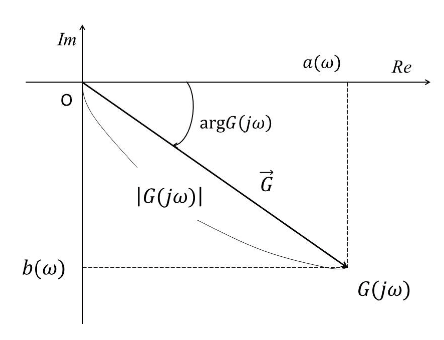
\includegraphics[width=0.5\linewidth]{picture/G_1.png}
  \caption{周波数伝達関数\\出典:永田正伸(2020), 1ページ\cite{text}}
  \label{P:G_1}
\end{figure}

\subsection{ベクトル軌跡}
図\ref{P:G_1}で示した$\overleftrightarrow{G}$において,周波数$\omega$を$0\sim +\infty$まで変化させたとき,ベクトルの
先端が軌跡を描く.これをベクトル軌跡という.また,周波数$\omega$を$-\infty \sim +\infty$に変化させたときに描く軌跡をナイキスト
軌跡(図\ref{P:G_2})という.
\begin{figure}[H]
  \centering
  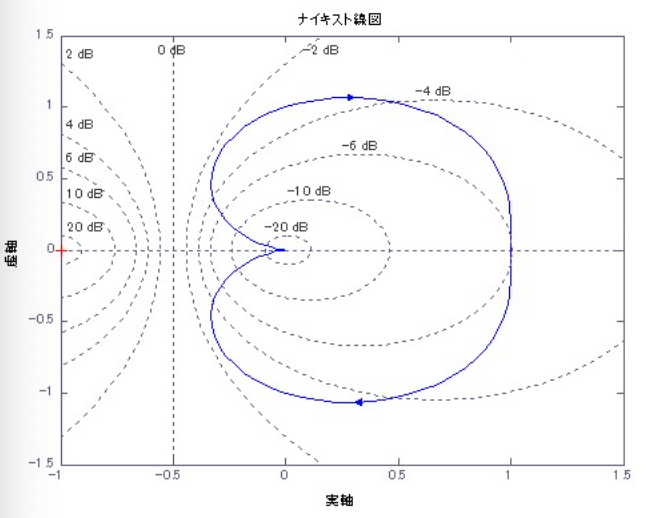
\includegraphics[width=0.5\linewidth]{picture/G_2.png}
  \caption{ナイキスト線図\\出典:永田正伸(2020), 2ページ\cite{text}}
  \label{P:G_2}
\end{figure}

\subsection{ボード線図}
ボード線図(図\ref{P:G_3})とは,ゲインと位相についてそれぞれ片対数でグラフにしたものである.ゲインについては,デシベル値$20\log_{10}|G(j\omega)|$
によるゲイン曲線で表しており,位相については,度[deg]による位相曲線で表す.\\
ボード線図において,伝達関数$G(s)$が複数($k$個)の伝達関数の積で表されるとき,
\begin{eqnarray}
  20\log_{10}|G(j\omega)| &=& \sum_{i=1}^{k}20\log_{10}|G_i(j\omega)| \\
  argG(j\omega) &=& \sum_{i=1}^{k}argG_i(j\omega)
\end{eqnarray}
が成り立つ.このとこから,高次の伝達関数の周波数特性を低次の伝達関数の要素で得ることができることが
ボード線図の特徴の一つである.
\begin{figure}[H]
  \centering
  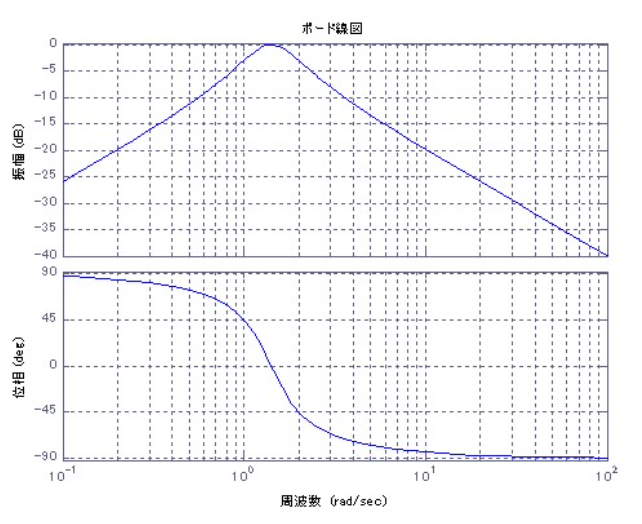
\includegraphics[width=0.5\linewidth]{picture/G_3.png}
  \caption{ボード線図\\出典:永田正伸(2020), 2ページ\cite{text}}
  \label{P:G_3}
\end{figure}

\section{実験}
\subsection{一次遅れ系の正弦波応答}
\begin{enumerate}
  \item ラプラス変換を用いて$y(t)$を導出する.\cite{junbi2}\\
        動的システム\\
        \begin{eqnarray}
          Y(s) = P(s)U(s) \label{Ys1}
          P(s)=\frac{1}{s+1} \label{Ps1}
        \end{eqnarray}
        において,入力を\\
        \[u(t)=A\sin{\omega t} \quad (A>0, \omega>0)\]
        としたときの出力$y(t)$を調べる.\\
        まず,ラプラス変換を用いて$U(s)$を求めると,
        \begin{equation}
          U(s) = \mathcal{L}[A\sin{\omega t}] = \frac{A\omega}{s^2+\omega^2} \label{Us1}
        \end{equation}
        式\ref{Ys1}に式\ref{Ps1},\ref{Us1}を代入すると,
        \begin{equation}
          Y(s) = \frac{1}{s+1}\cdot \frac{A\omega}{s^2+\omega^2}=\frac{A\omega}{(s+1)(s^2+\omega^2)} \label{Ys2}
        \end{equation}
        ここで上式\ref{Ys2}を部分分数分解する.任意定数を$a$,$b$,$c$とすると,
        \begin{equation}
          \frac{A\omega}{(s+1)(s^2+\omega^2)} = \frac{a}{s+1}+\frac{bs+c}{s^2+\omega^2}=\frac{a(s^2+\omega^2)+(s+1)(bs+c)}{(s+1)(s^2+\omega^2)}\nonumber
        \end{equation}
        両辺の分子を係数比較すると,
        \begin{eqnarray}
          A\omega &=& a(s^2+\omega^2)+(s+1)(bs+c)\\ \nonumber
          &=& as^2+a\omega^2+bs^2+cs+bs+c \\ \nonumber
          &=& (a+b)s^2 + (b+c)s + a\omega^2+c \label{Aw1}
        \end{eqnarray}
        式\ref{Aw1}より,以下の連立方程式を立てることができる.
        \begin{equation}
          \left\{ \,
          \begin{aligned}
             & a + b = 0               \\
             & b + c = 0               \\
             & a\omega^2 + c = A\omega
          \end{aligned}
          \right.
          \label{abc}
        \end{equation}
        式\ref{abc}を解くと,$a=\frac{A\omega}{\omega^2+1}$,$b=-\frac{A\omega}{\omega^2+1}$,$\frac{A\omega}{\omega^2+1}$
        となる.よって$Y(s)$は,
        \begin{equation}
          Y(s) = \frac{A\omega}{(\omega^2+1)(s+1)} - \frac{A\omega s}{(\omega^2+1)(s^2+\omega^2)} + \frac{A\omega}{(\omega^2+1)(s^2+\omega^2)} \label{Ys3}
        \end{equation}
        式\ref{Ys3}を逆ラプラス変換を用いて$y(t)$の式に変換すると,
        \begin{eqnarray}
          y(t) &=& \mathcal{L}^{-1}[Y(s)] = \mathcal{L}^{-1}\left[\frac{A\omega}{(\omega^2+1)(s+1)}\right]-\mathcal{L}^{-1}\left[\frac{A\omega s}{(\omega^2+1)(s^2+\omega^2)}\right] + \mathcal{L}^{-1}\left[\frac{A\omega}{(\omega^2+1)(s^2+\omega^2)}\right] \nonumber \\
          &=&  \frac{A\omega}{\omega^2+1}\cdot e^{-t} - \frac{A\omega}{\omega^2+1}\cdot \cos{\omega t} + \frac{A}{\omega^2 + 1} \cdot \sin{\omega t} \nonumber \\
          &=& \frac{A\omega}{\omega^2+1}\cdot e^{-t} + \frac{A}{1+\omega^2}(\sin{\omega t}-\omega\cos{\omega t}) \label{Yt1}
        \end{eqnarray}

  \item $y_{ss}$の導出\\
        次に,定常状態での出力$y_{ss}(t)$について調べる.定常状態では十分に時間が経過していることを指し,$t$の値は大きくなっているため,
        \begin{equation}
          \lim_{t\rightarrow\infty}e^{-t}=0 \label{e_0}
        \end{equation}
        が成り立つことがわかる.上記の式\ref{e_0}より,式\ref{Yt1}の第一項は無視できることがわかる.
        さらに,ここで三角関数の合成
        \begin{equation}
          a\sin{\omega t}+b\cos{\omega t} = \sqrt{a^2+b^2}\sin{\omega t + \phi} \nonumber
        \end{equation}
        を用いると,
        \begin{eqnarray}
          y_{ss}(t) &=& \frac{A}{1+\omega^2}(\sin{\omega t}-\omega\cos{\omega t}) \nonumber \\
          &=& \frac{A}{1+\omega^2} \cdot \sqrt{1+\omega^2}\sin{\omega t + \phi(\omega)} \nonumber \\
          &=& \frac{A}{\sqrt{1+\omega^2}}\sin({\omega t + \phi(\omega)})
        \end{eqnarray}
        $\frac{A}{\sqrt{1+\omega^2}} = B(\omega)$と置くと,
        \begin{equation}
          Y_{ss}(t) = B(\omega)\sin{(\omega t - \omega \cos{\omega t})}
        \end{equation}
        と導出することができる.

  \item $A=1$,$\omega = 0.5, 1, 50$としたときの波形$u(t)$,$y(t)$および$y_{ss}(t)$をScilabを用いて計算してプロットする.\\
        以下にグラフをプロットするためのソースコード\ref{C:3-1-1-05},\ref{C:3-1-1-1},\ref{C:3-1-1-50}を示し,その結果を図\ref{3-1-1-05},\ref{3-1-1-1},\ref{3-1-1-50}に示す.
        グラフは,グレーが$u(t)$,緑が$y(t)$,青が$y_{ss}(t)$となっている.
        \begin{lstlisting}[caption=図\ref{3-1-1-05}をプロットするコード, label=C:3-1-1-05]
s = %s;
P = syslin('c',1/(s+1))
t = 0:0.01:20;
A = 1;
Omeg = 0.5;
u = A*sin(Omeg*t);
y = csim(u,t,P);
yss = A/(1+Omeg*Omeg)*(sin(Omeg*t)-Omeg*cos(Omeg*t));
plot2d(t,u,style=color(125,125,125));
plot2d(t,y,style=3);
plot2d(t,yss,style=2);
xtitle("Frequency Response","time[s]","u,y,yss");
xgrid();
      \end{lstlisting}
        \begin{figure}[H]
          \centering
          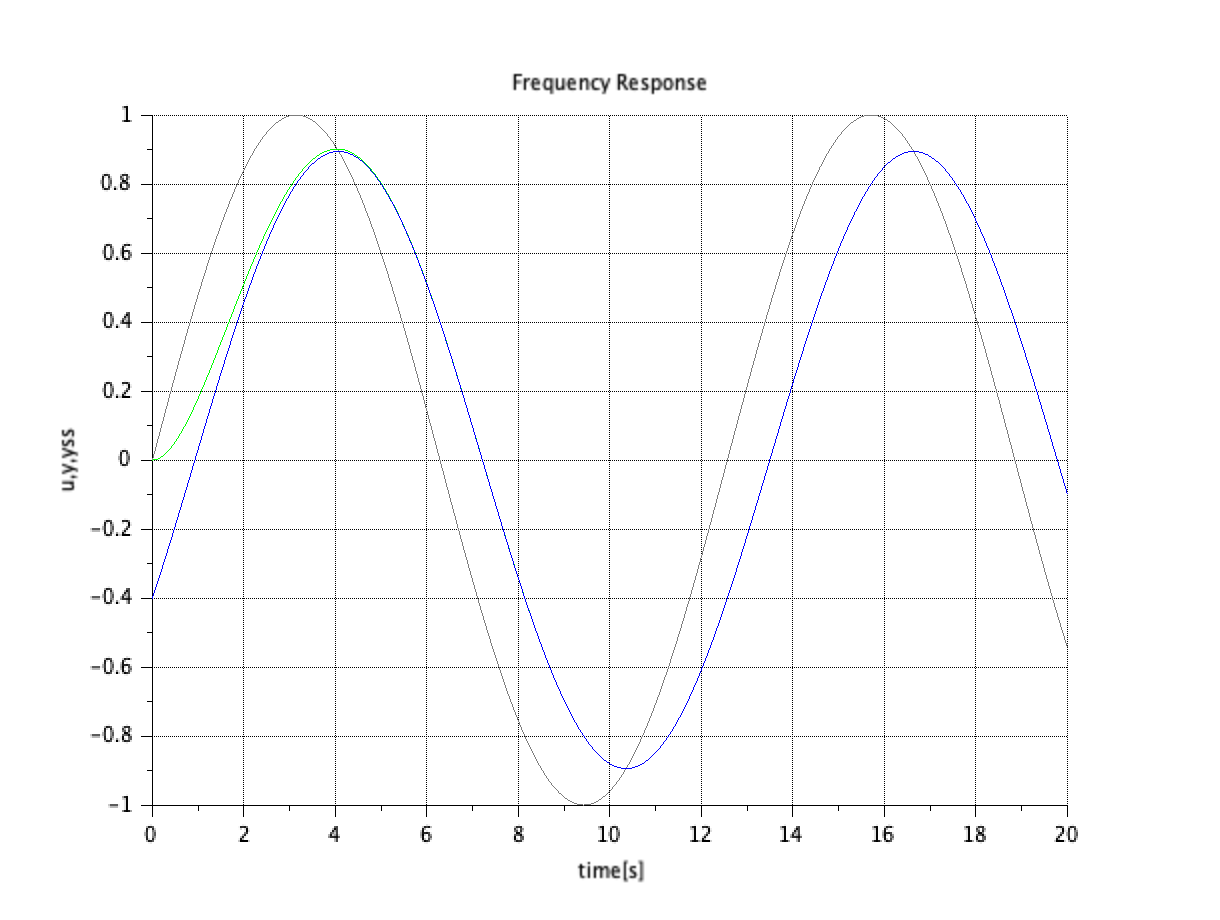
\includegraphics[width=0.8\linewidth]{picture/3-1-1-05.png}
          \caption{$\omega=0.5$のとき}
          \label{3-1-1-05}
        \end{figure}
        \begin{lstlisting}[caption=図\ref{3-1-1-1}をプロットするコード, label=C:3-1-1-1]
s = %s;
P = syslin('c',1/(s+1))
t = 0:0.01:20;
A = 1;
Omeg = 1;
u = A*sin(Omeg*t);
y = csim(u,t,P);
yss = A/(1+Omeg*Omeg)*(sin(Omeg*t)-Omeg*cos(Omeg*t));
plot2d(t,u,style=color(125,125,125));
plot2d(t,y,style=3);
plot2d(t,yss,style=2);
xtitle("Frequency Response","time[s]","u,y,yss");
xgrid();
      \end{lstlisting}
        \begin{figure}[H]
          \centering
          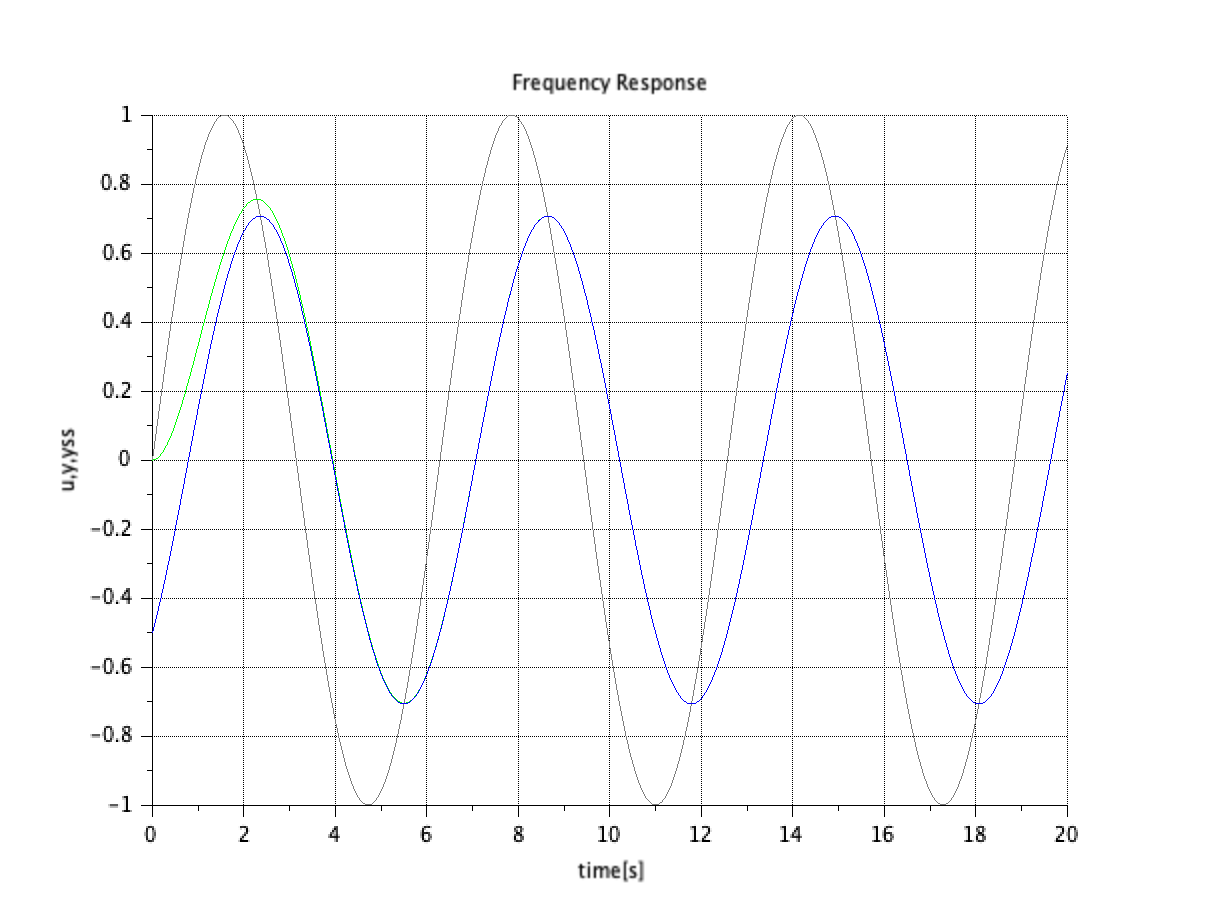
\includegraphics[width=0.8\linewidth]{picture/3-1-1-1.png}
          \caption{$\omega=1$のとき}
          \label{3-1-1-1}
        \end{figure}

        \begin{lstlisting}[caption=図\ref{3-1-1-50}をプロットするコード, label=C:3-1-1-50]
s = %s;
P = syslin('c',1/(s+1))
t = 0:0.01:20;
A = 1;
Omeg = 50;
u = A*sin(Omeg*t);
y = csim(u,t,P);
yss = A/(1+Omeg*Omeg)*(sin(Omeg*t)-Omeg*cos(Omeg*t));
plot2d(t,u,style=color(125,125,125));
plot2d(t,y,style=3);
plot2d(t,yss,style=2);
xtitle("Frequency Response","time[s]","u,y,yss");
xgrid();
      \end{lstlisting}
        \begin{figure}[H]
          \centering
          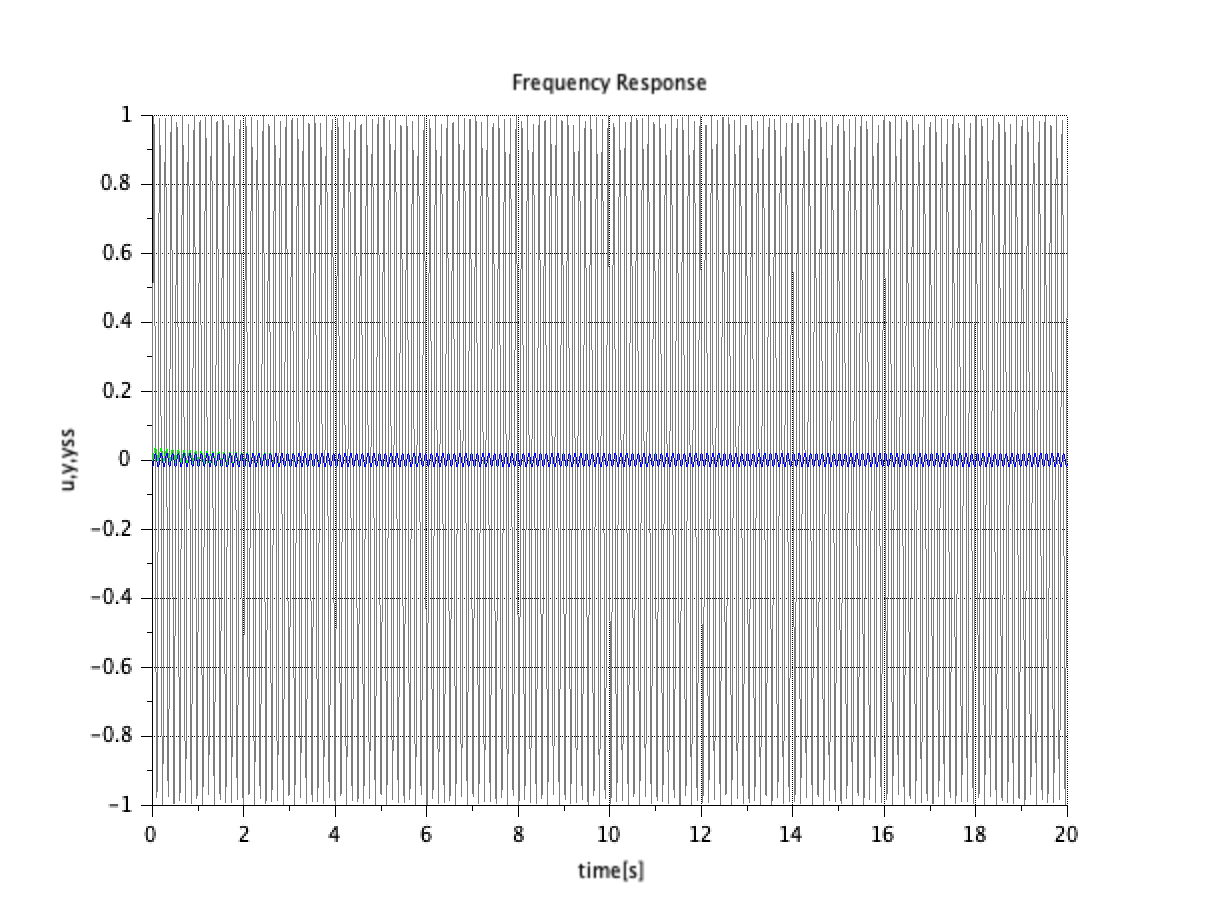
\includegraphics[width=0.8\linewidth]{picture/3-1-1-50.png}
          \caption{$\omega = 50$のとき}
          \label{3-1-1-50}
        \end{figure}
        グラフより,周波数$\omega$が大きくなればゲインは小さくなり,位相がさらに遅れていることが
        わかる.これは,$B(\omega)$において,分母の値が$\omega$について変化していることからもわかる.
\end{enumerate}

\subsection{二次遅れ系の正弦波応答}
伝達関数$P(s)$が$P(s) = \frac{1}{s^2+1.4s+1}$で与えられたとき,$A=1$,$\omega = 0.5$,$1$,$50$とした場合
の時間応答をScilabを用いてプロットする.以下に作成したソースコード\ref{C:3-1-2}とその実行結果(図\ref{3-1-2-05},\ref{3-1-2-1},\ref{3-1-2-50})を示す.
\begin{lstlisting}[caption=二次遅れ系の正弦波応答, label=C:3-1-2]
clear();
clc();
s = %s;
P = syslin('c',1/(s*s+1.4*s+1))
t = 0:0.01:20;
A = 1;
Omeg = 0.5;
u = A*sin(Omeg*t);
y = csim(u,t,P);
yss = A/(1+Omeg*Omeg)*(sin(Omeg*t)-Omeg*cos(Omeg*t));
scf(0);
plot2d(t,u,style=color(125,125,125));
plot2d(t,y,style=3);
plot2d(t,yss,style=2);
xtitle("Frequency Response","time[s]","u,y,yss");
xgrid();
xs2png(0, 'Omeg.png')
    \end{lstlisting}
\begin{figure}[H]
  \begin{tabular}{cc}
    \begin{minipage}[t]{0.48\textwidth}
      \centering
      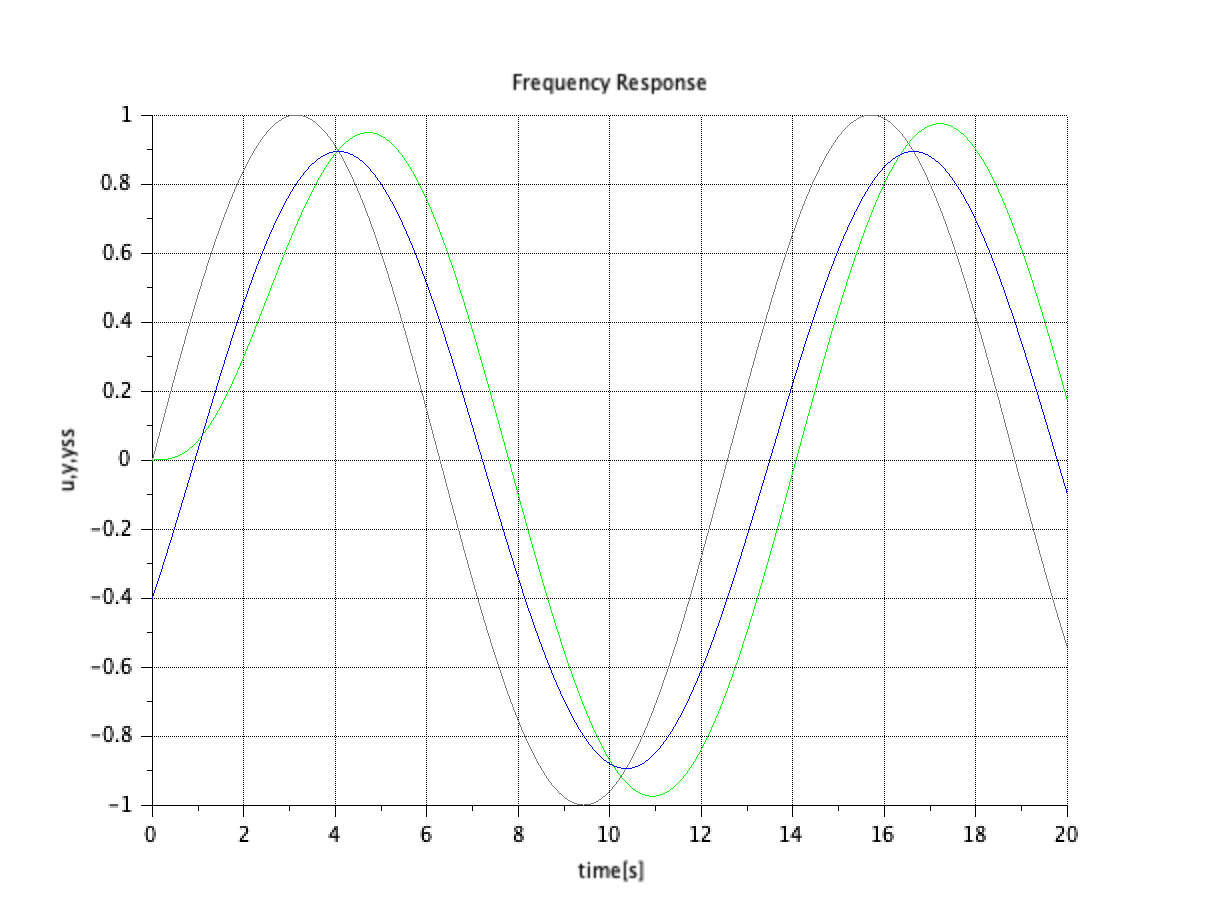
\includegraphics[clip,width=9cm]{picture/3-1-2-05.png}
      \caption{$\omega = 0.5$のとき}
      \label{3-1-2-05}
    \end{minipage} &
    \begin{minipage}[t]{0.48\textwidth}
      \centering
      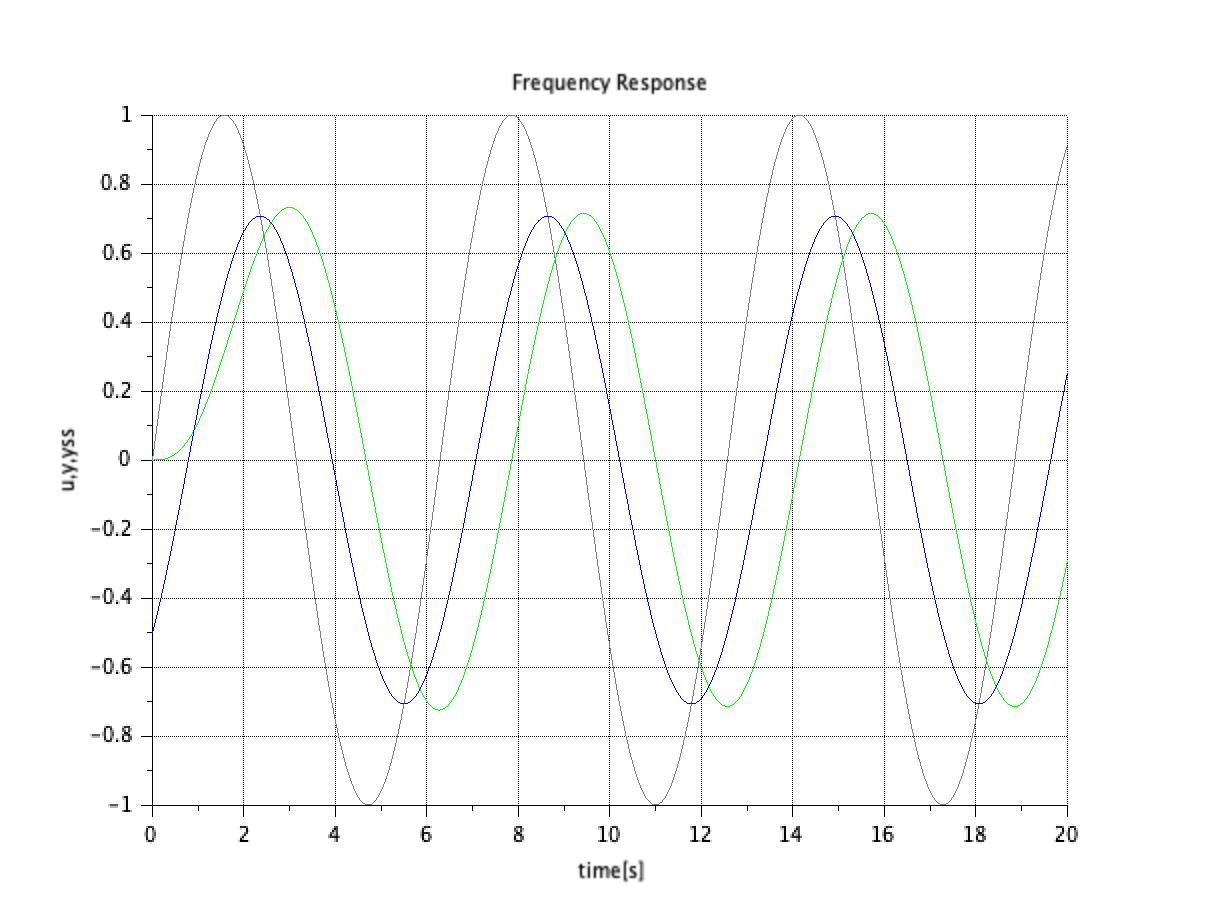
\includegraphics[clip,width=9cm]{picture/3-1-2-1.png}
      \caption{$\omega = 1$のとき}
      \label{3-1-2-1}
    \end{minipage}
  \end{tabular}
\end{figure}
\begin{figure}[H]
  \centering
  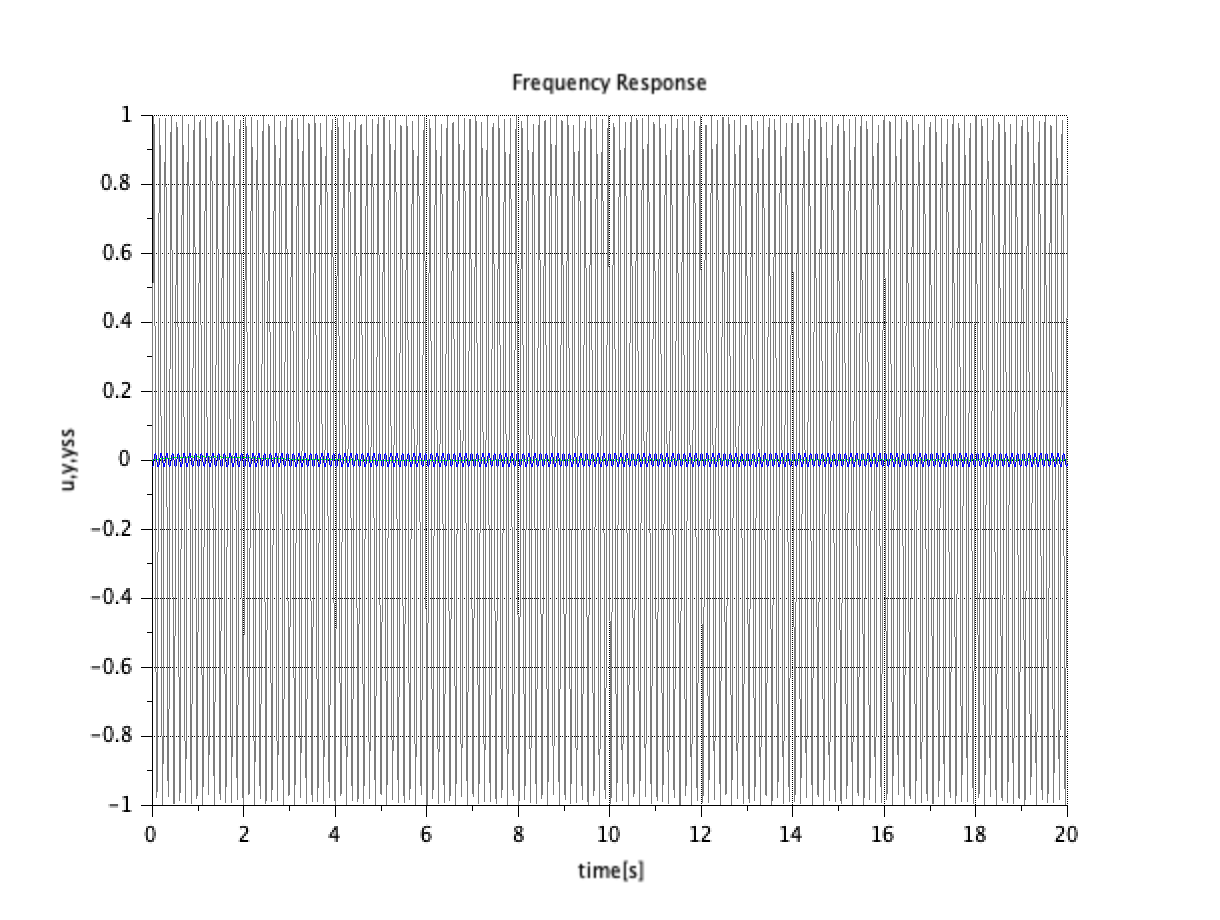
\includegraphics[width=9cm]{picture/3-1-2-50.png}
  \caption{$\omega = 50$のとき}
  \label{3-1-2-50}
\end{figure}
グラフからわかるように,周波数$\omega$に対するゲインと位相の関係は一次遅れ系と変わらなかったが,
二次遅れ系については,出力$y(t)$と定常状態での出力$y_{ss}(t)$に位相のズレが生じている.

\subsection{ベクトル軌跡}
二次遅れ系で与えられる伝達関数$P(s) = \frac{K\omega^2_n}{s^2+2\zeta\omega_ns+\omega^2_n}$の,
ゲイン定数$K$,減衰係数$\zeta$,固有角周波数$\omega_n$の変化を確認する.
\begin{enumerate}
  \item $K=1$,$\omega_n = 1$と固定して,$\zeta = 0.25, 0.5, 1$と変化させたときのナイキスト線図をプロットする.\\

        Scilabで作成したソースコード\ref{C:3-2-1}とその実行結果(図\ref{3-2-1})を以下に示す.
        \begin{lstlisting}[caption=二次遅れ系のナイキスト線図, label=C:3-2-1]
clear();
clc();
s = %s;
scf(0);
K = 1;
Omeg = 1;

zeta = 0.25;
P1 = syslin('c',K*Omeg*Omeg/(s*s+2*zeta*Omeg*s+Omeg*Omeg));

zeta = 0.5;
P2 = syslin('c',K*Omeg*Omeg/(s*s+2*zeta*Omeg*s+Omeg*Omeg));

zeta = 1;
P3 = syslin('c',K*Omeg*Omeg/(s*s+2*zeta*Omeg*s+Omeg*Omeg));

nyquist([P1;P2;P3],%t);
xs2png(0, 'nyquist1.png')
      \end{lstlisting}
        \begin{figure}[H]
          \centering
          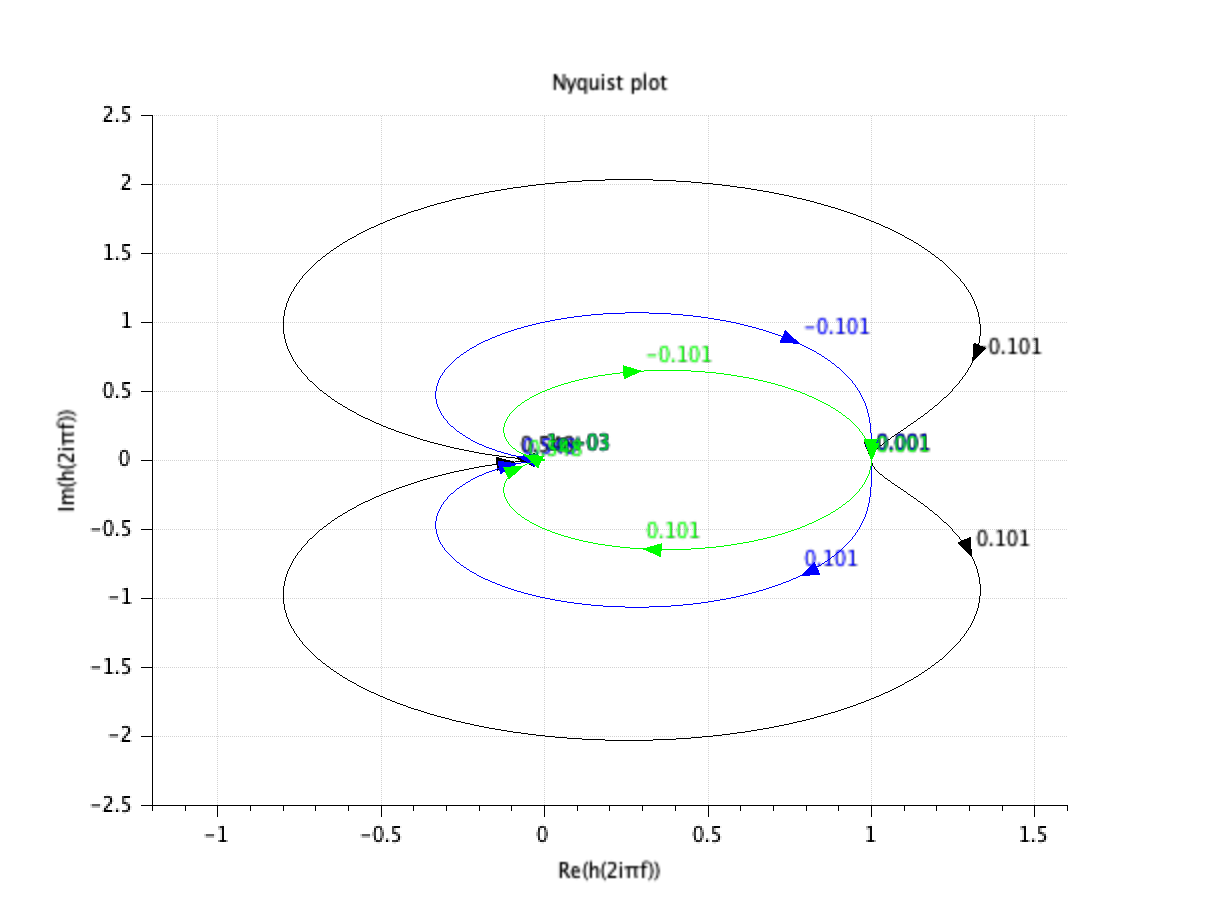
\includegraphics[width=0.8\linewidth]{picture/3-2-1.png}
          \caption{ナイキスト線図($\omega=0.25(黒)$,$\omega = 0.5(青)$,$\omega = 1(緑)$)}
          \label{3-2-1}
        \end{figure}

  \item 二次遅れ系の正弦波応答の実験で作成したソースコード\ref{C:3-1-2}を用いて,
        減衰係数$\zeta$と角周波数$\omega$をそれぞれ変化させたときのベクトル軌跡の変化を確認する.\\
        以下の表\ref{T:3-2-2}に出力結果を整理して示す.
        \newpage
        \begin{table}[H]
          \centering
          \caption{減衰係数$\zeta$と角周波数$\omega$を変化させたときの実験結果}
          \begin{tabular}{|c|c|c|c|c|} \hline
            \multicolumn{2}{|c|}{\multirow{2}{*}{実験結果}}
             &
            \multicolumn{3}{|c|}{$\zeta$}
            \\ \cline{3-5}


             &

             &
            0.25
             &
            0.5
             &
            1
            \\ \hline

            \multirow{6}{*}{$\omega$}
             &
            \multirow{2}{*}{0.1}
             &
            \begin{minipage}{45mm}
              \centering
              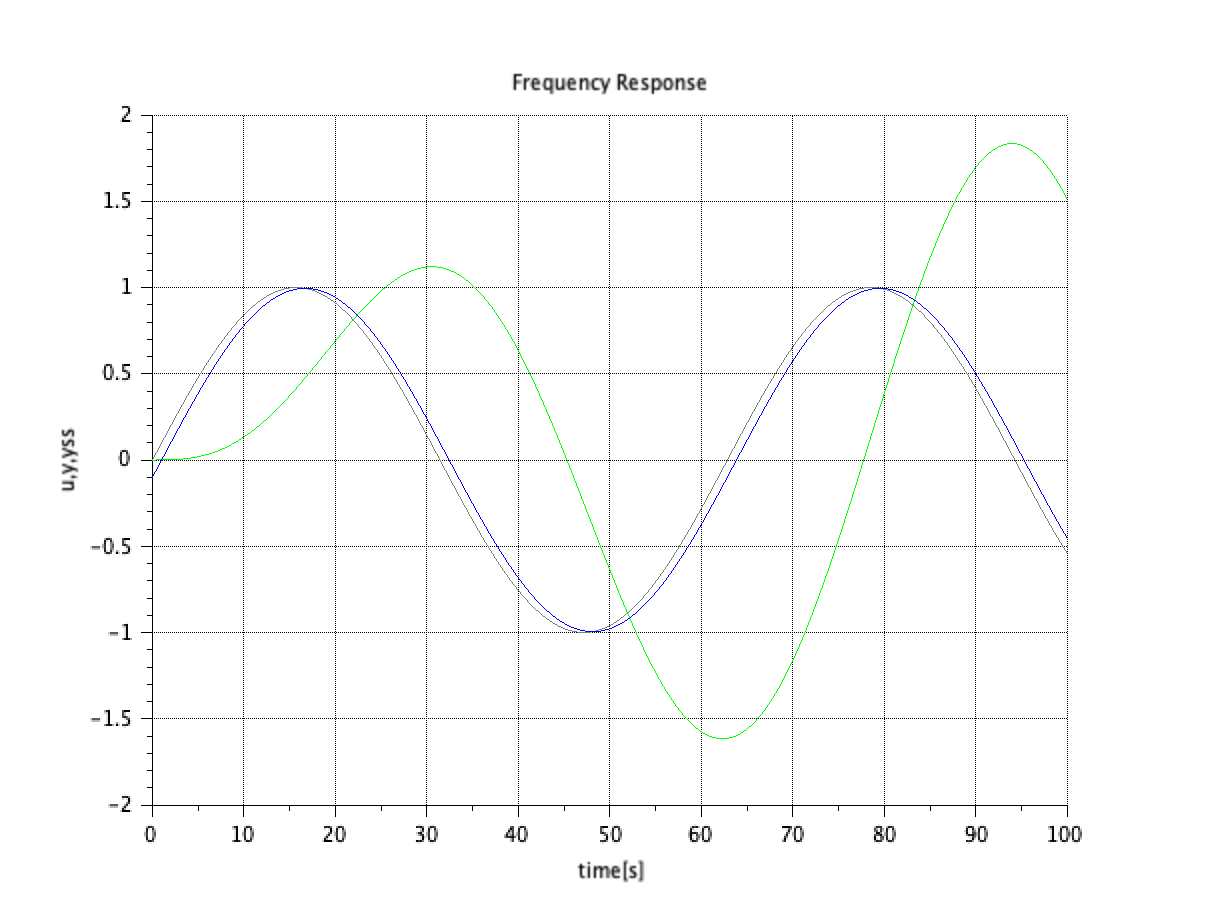
\includegraphics[width=3cm,clip]{picture/1.png}
            \end{minipage}
             &
            \begin{minipage}{45mm}
              \centering
              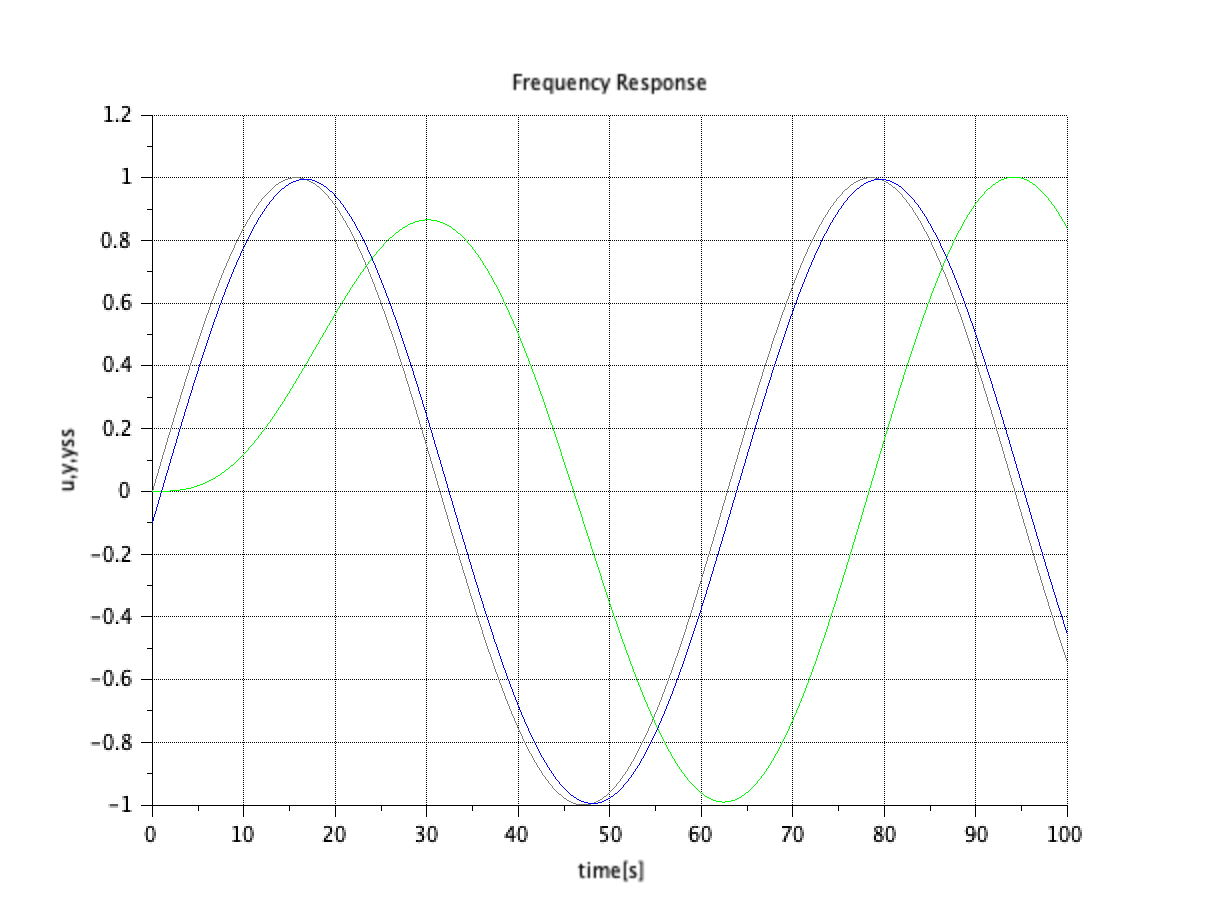
\includegraphics[width=3cm,clip]{picture/4.png}
            \end{minipage}
             &
            \begin{minipage}{45mm}
              \centering
              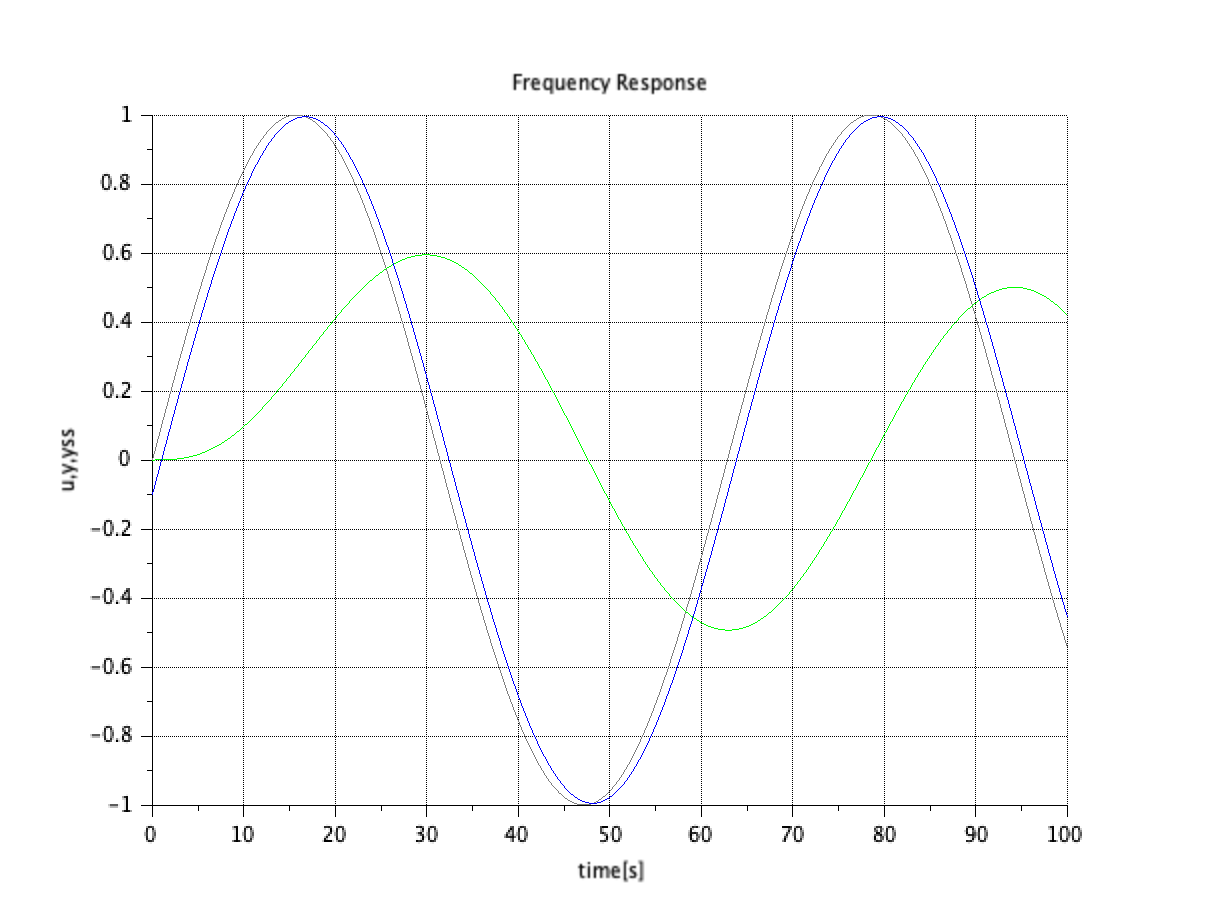
\includegraphics[width=3cm,clip]{picture/7.png}
            \end{minipage}
            \\ \cline{3-5}


             &

             &
            ゲイン:1.位相:5.71(遅れ)
             &
            ゲイン:1,位相:5.71(遅れ)
             &
            ゲイン:1,位相:5.71(遅れ)
            \\\cline{2-5}


             &
            \multirow{2}{*}{0.5}
             &
            \begin{minipage}{45mm}
              \centering
              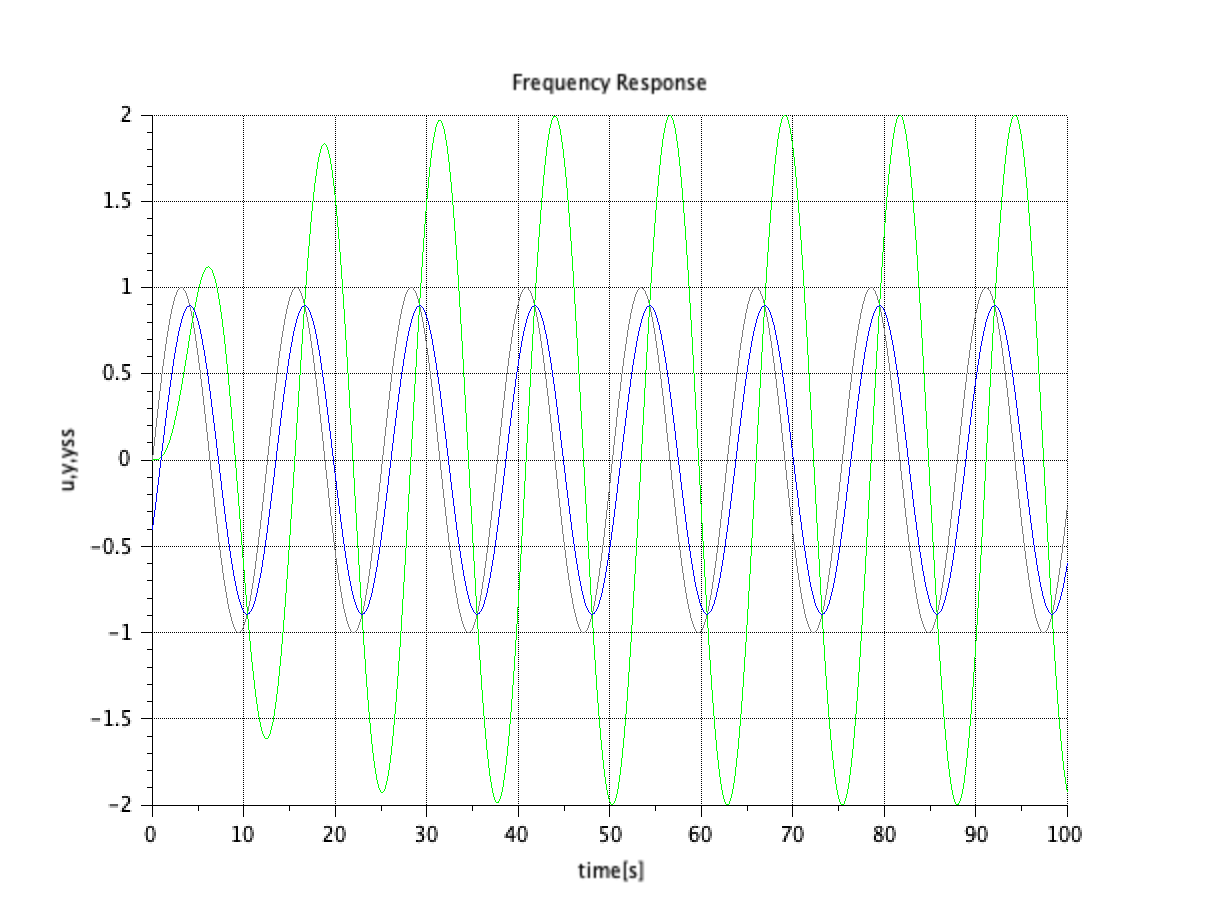
\includegraphics[width=3cm,clip]{picture/2.png}
            \end{minipage}
             &
            \begin{minipage}{45mm}
              \centering
              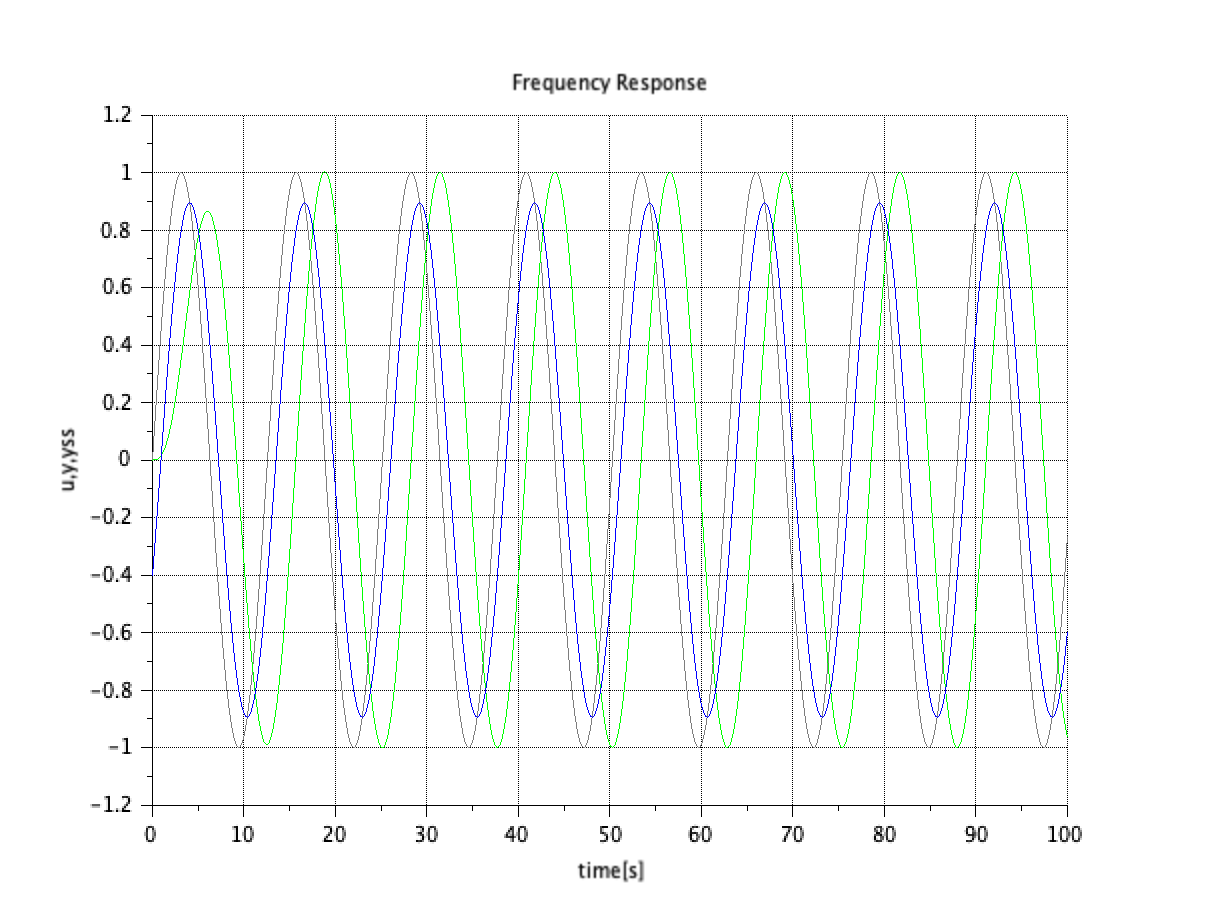
\includegraphics[width=3cm,clip]{picture/5.png}
            \end{minipage}
             &
            \begin{minipage}{45mm}
              \centering
              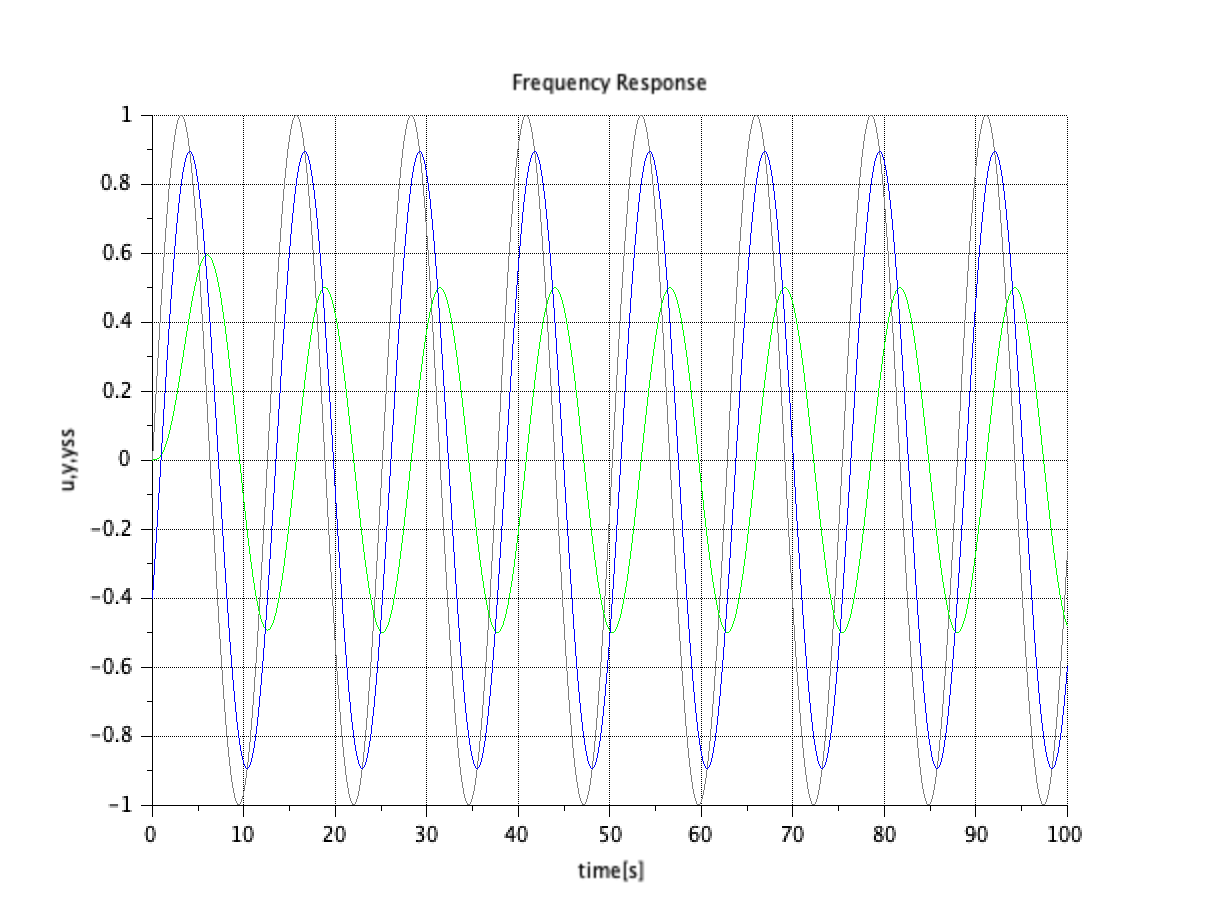
\includegraphics[width=3cm,clip]{picture/8.png}
            \end{minipage}
            \\\cline{3-5}


             &

             &
            ゲイン:0.89,位相:26.57(遅れ)
             &
            ゲイン:0.89,位相:26.57(遅れ)
             &
            ゲイン:0.89,位相:26.57(遅れ)
            \\\cline{2-5}


             &
            \multirow{2}{*}{1}
             &
            \begin{minipage}{45mm}
              \centering
              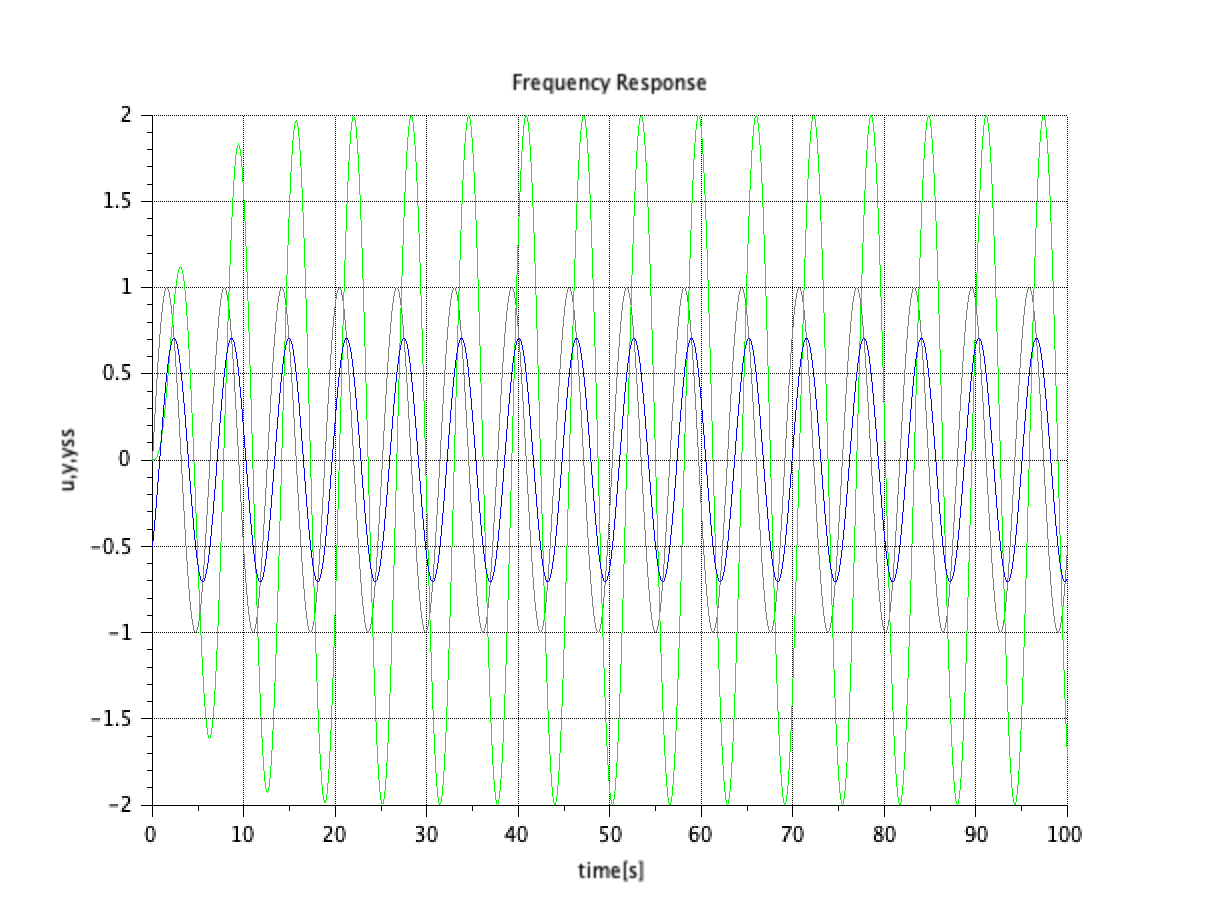
\includegraphics[width=3cm,clip]{picture/3.png}
            \end{minipage}
             &
            \begin{minipage}{45mm}
              \centering
              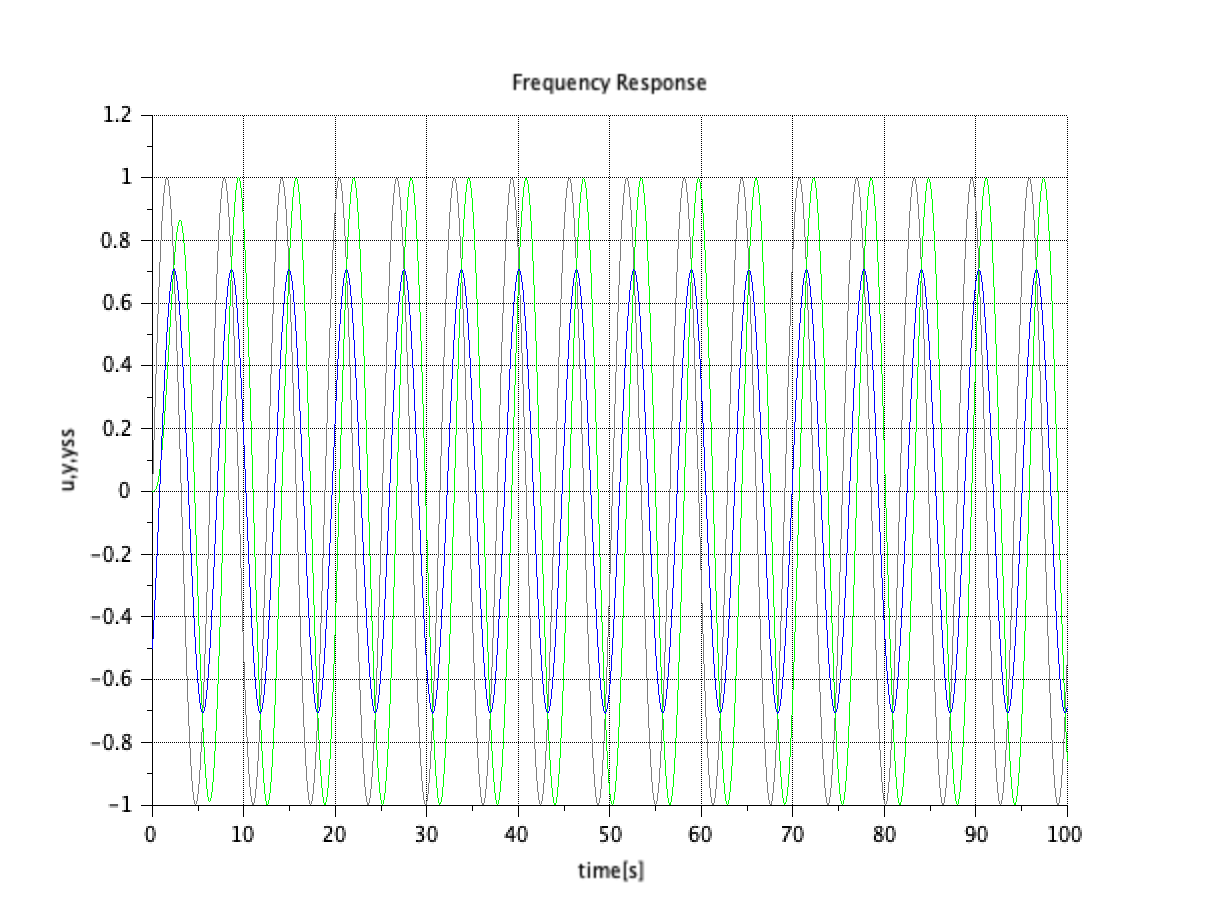
\includegraphics[width=3cm,clip]{picture/6.png}
            \end{minipage}
             &
            \begin{minipage}{45mm}
              \centering
              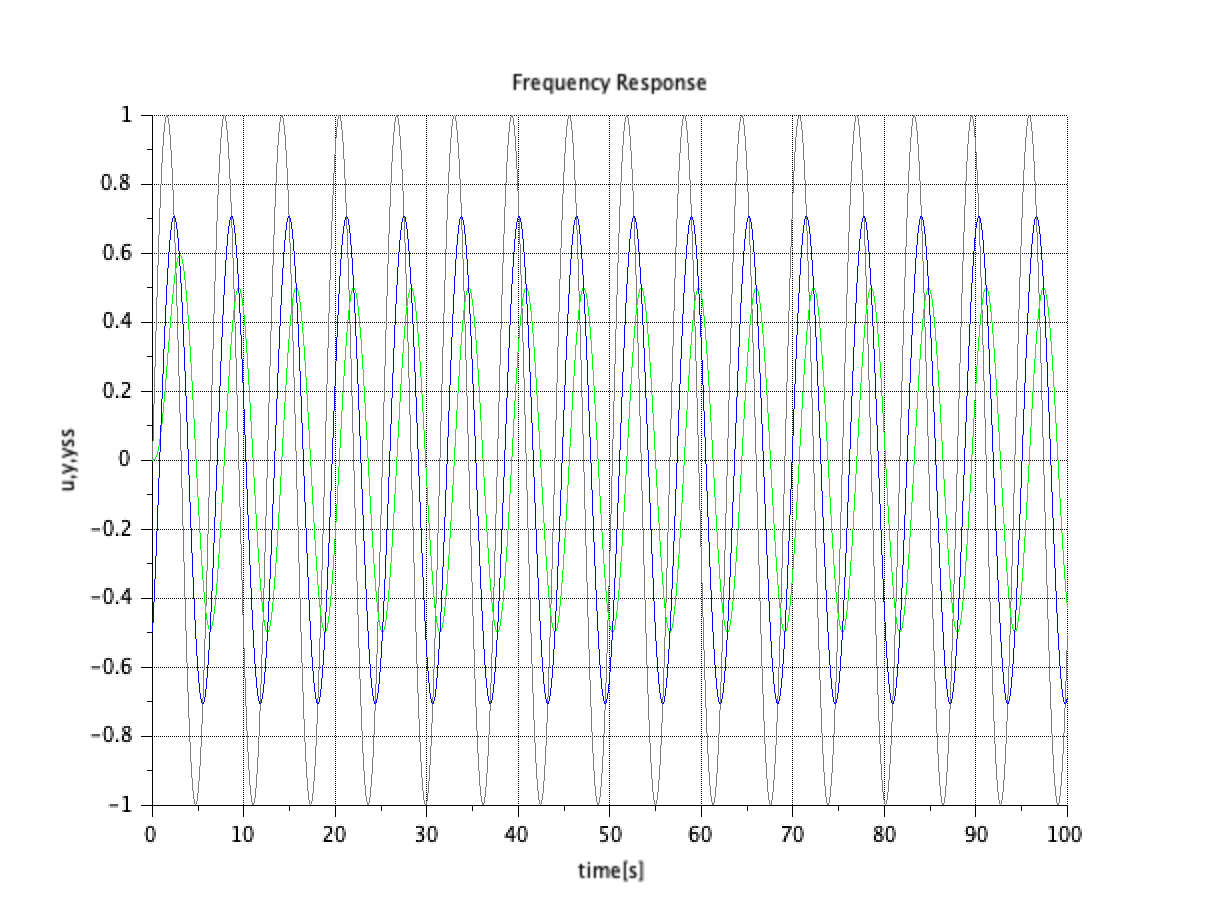
\includegraphics[width=3cm,clip]{picture/9.png}
            \end{minipage}
            \\\cline{3-5}


             &

             &
            ゲイン:0.7,位相:45(遅れ)
             &
            ゲイン:0.7,位相:45(遅れ)
             &
            ゲイン:0.7,位相:45(遅れ)
            \\\hline
          \end{tabular}
          \label{T:3-2-2}
        \end{table}
\end{enumerate}

\subsection{ボード線図}
\subsubsection{ボード線図の作成}
\begin{enumerate}
  \item
        二次遅れ系で与えられた伝達関数$P(s)=\frac{K\omega^2_n}{s^2+2\zeta\omega_ns+\omega^2_n}$において,$K=1$,
        $\omega_n=1$と固定し,$\zeta=0.25,0.5,1$と変化させたときの$P(s)$の周波数応答特性を表すボード線図を,
        角周波数$\omega=0.01 \sim 100$と指定してプロットする.そのときに作成したソースコード\ref{C:3-3-1-1}とその実行結果(図\ref{3-3-1-1})を
        以下に示す.
        \begin{lstlisting}[caption=C:3-3-1-1]
  clear();
  clc();
  scf(0);
  s = %s;
  Omeg = 1;
  zeta = 0.25;
  G1 = Omeg*Omeg/(s^2+2*zeta*Omeg*s+Omeg*Omeg);
  P1 = syslin('c',G1);
  Peak_freq1 = freson(P1)
  w_freq1 = 2*%pi*Peak_freq1
  Max_G1 = 20*log10(abs(horner(G1,%i*w_freq1)))


  zeta = 0.5;
  G2 = Omeg*Omeg/(s^2+2*zeta*Omeg*s+Omeg*Omeg);
  P2 = syslin('c',G2);
  Peak_freq2 = freson(P2)
  w_freq2 = 2*%pi*Peak_freq2
  Max_G2 = 20*log10(abs(horner(G2,%i*w_freq2)))

  zeta = 1.0;
  G3 = Omeg*Omeg/(s^2+2*zeta*Omeg*s+Omeg*Omeg);
  P3 = syslin('c',G3);
  Peak_freq3 = freson(P3)
  w_freq3 = 2*%pi*Peak_freq3
  Max_G3 = 20*log10(abs(horner(G3,%i*w_freq3)))

  xset('window',0);
  bode([P1;P2;P3]);

  disp(Peak_freq1)
  disp(w_freq1)
  disp(Max_G1)
  disp(Peak_freq2)
  disp(w_freq2)
  disp(Max_G2)
  disp(Peak_freq3)
  disp(w_freq3)
  disp(Max_G3)

  //xs2png(0, 'kadai6.png')
      \end{lstlisting}
        \begin{figure}[H]
          \centering
          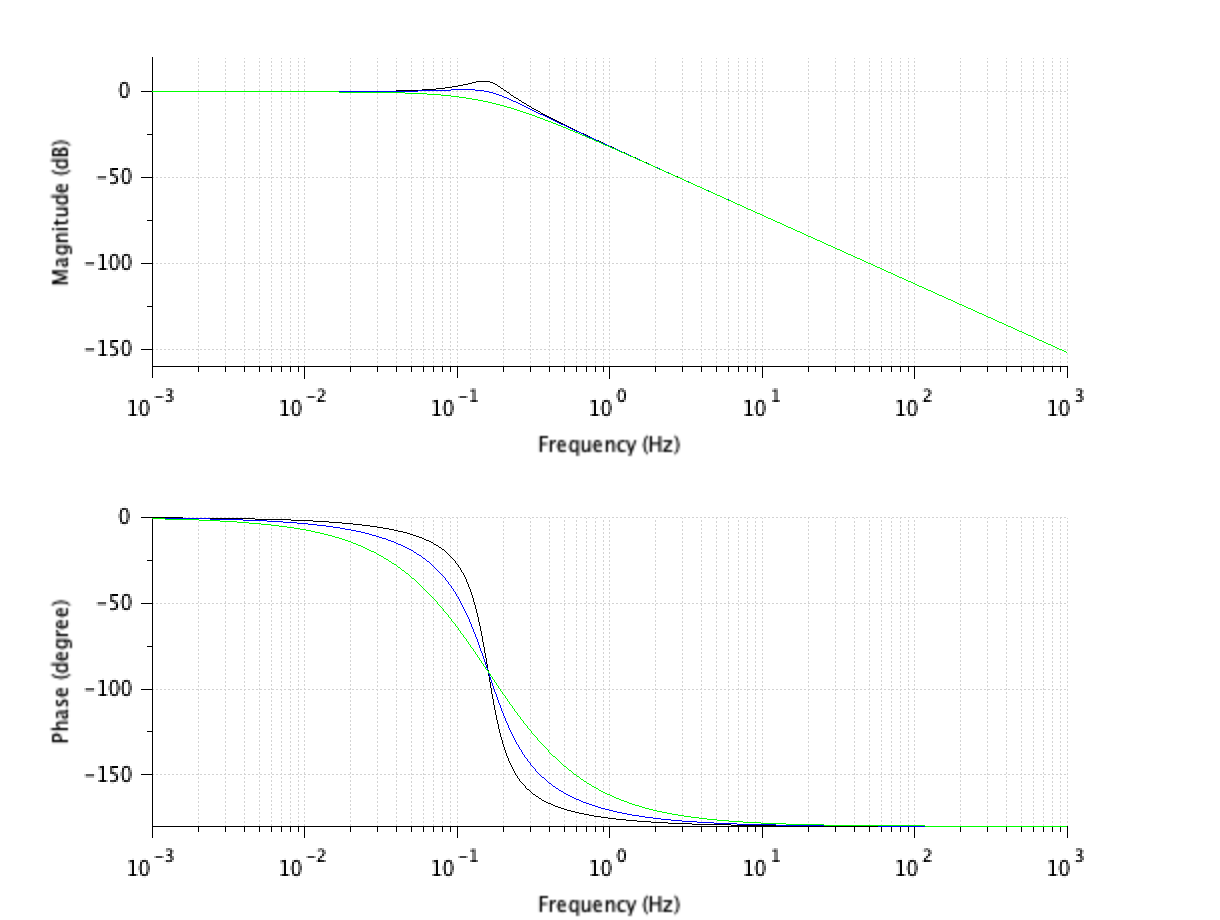
\includegraphics[width=0.8\linewidth]{picture/kadai6.png}
          \caption{ボード線図($\zeta=0.25$(黒),$\zeta=0.5$(青),$\zeta=1(緑)$)}
          \label{3-3-1-1}
        \end{figure}
  \item
        設定した周波数域内でゲインが最大となるピーク周波数$\omega_p$
        と,そのときのゲインの値(共振ピーク)$M_p$をScilabにより算出し記録する.\\
        以下そにScilabで算出した$\omega_p$と$M_p$の結果である.\\
        $\zeta=0.25$のとき$\cdots \omega_p=0.1488758$,\qquad $M_p=6.3008871$ \\
        $\zeta=0.5$のとき$\cdots \omega_p=0.1125395$,\qquad $M_p=1.2493874$ \\
        $\zeta=1$のとき$\cdots \omega_p=[]$,\qquad $M_p=[]$ \\

  \item 実験4.3.2の結果と比較してボード線図の特徴との対応を考察する.\\
        表\ref{T:3-2-2}で示した結果と比較すると,
        図\ref{3-3-1-1}で示したボード線図のほうが,視覚的に得ることができる
        $\omega$に対する情報が明確でありそれがボード線図の特徴である.
        $\zeta=0.25,0.5$のとき,$\omega_p$と$M_p$を求めることができたが,
        $\zeta=1$のときは求めることができなかった.これは,設定した周波数域内
        で最大値が存在していないからだと予測できる.
\end{enumerate}

\subsubsection{2つの伝達関数要素の直列結合とボード線図}
\begin{enumerate}
  \item 伝達関数$P(s)=\frac{s+0.1}{s+1}$のボード線図を描く.\\
        以下にScilabで作成したソースコード\ref{C:3-3-2-1}を示す.また,その実行結果を図\ref{3-3-2-1}に示す.
        \begin{lstlisting}[caption=図\ref{3-3-2-1}をプロットするコード, label=C:3-3-2-1]
clear();
clc();
s=%s;

P=(s+0.1)/(s+1);
P1=1/s+1;
P2=s+0.1;

w = logspace(-2,2,400);

Pjw = horner(P,%i*w);
[Phase,GaindB] = phasemag(Pjw,'c');
xset('window',0);
subplot(211);
plot2d(w,GaindB, logflag='ln', style=2);
xtitle('Bode Diagram','ω[rad/s]','Gain[dB]')
xgrid();
subplot(212);
plot2d(w,Phase, logflag='ln', style=2);
xtitle('', 'w[rad/s]','Phase[degree]')
xgrid();
      \end{lstlisting}
        \begin{figure}[H]
          \centering
          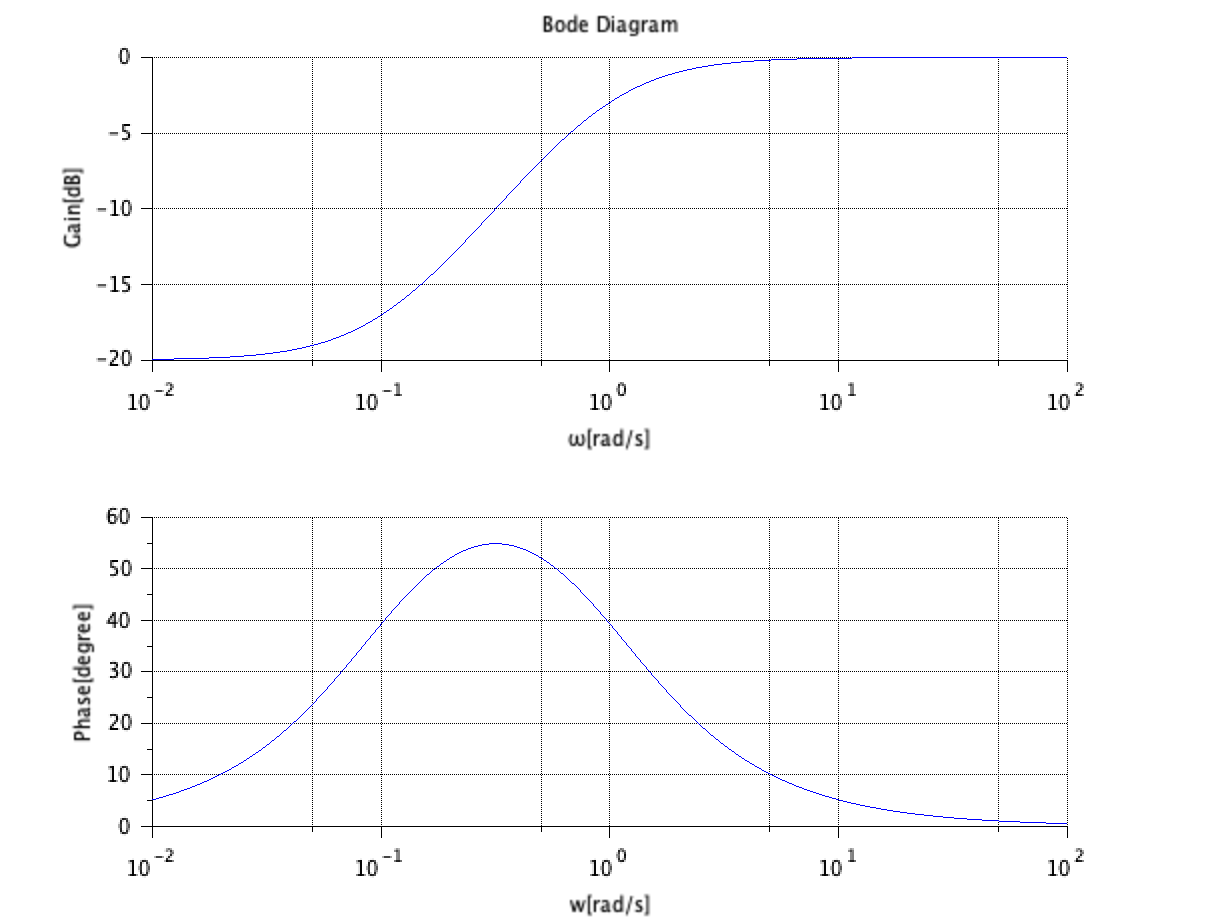
\includegraphics[width=0.8\linewidth]{picture/kadai7-1.png}
          \caption{$P(s)=\frac{s+0.1}{s+1}$のボード線図}
          \label{3-3-2-1}
        \end{figure}

  \item $P_1(s)=\frac{1}{s+1}$,$P_2(s)=s+0.1$のボード線図をそれぞれ描く.\\
        $P_1(s)=\frac{1}{s+1}$のボード線図をプロットするためのソースコード\ref{3-3-2-2-1}と実行結果(図\ref{3-3-2-2-1})を
        以下に示す.
        \begin{lstlisting}[caption=図\ref{3-3-2-2-1}をプロットするコード, label=C:3-3-2-2-1]
clear();
clc();
s=%s;

P=(s+0.1)/(s+1);
P1=1/s+1;
P2=s+0.1;

w = logspace(-2,2,400);
P1jw = horner(P1,%i*w);
[Phase1,GaindB1] = phasemag(P1jw,'c');
scf(1);
xset('window',1);
subplot(211);
plot2d(w,GaindB1, logflag='ln', style=2);
xtitle('Bode Diagram','ω[rad/s]','Gain[dB]')
xgrid();
subplot(212);
plot2d(w,Phase1, logflag='ln', style=2);
xtitle('', 'w[rad/s]','Phase[degree]')
xgrid();
      \end{lstlisting}
        \begin{figure}[H]
          \centering
          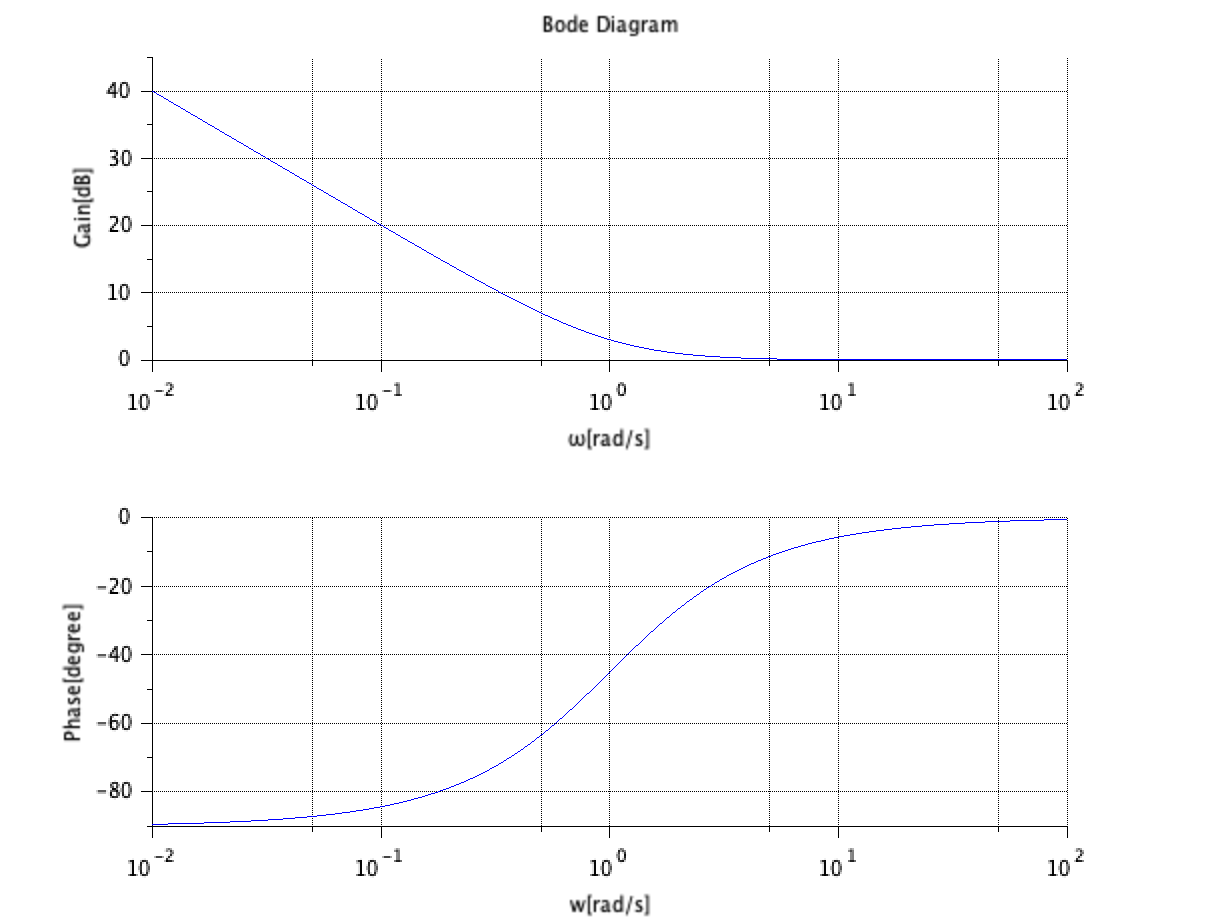
\includegraphics[width=0.8\linewidth]{picture/kadai7-2.png}
          \caption{$P_1(s)=\frac{1}{s+1}$のボード線図}
          \label{3-3-2-2-1}
        \end{figure}
        $P_2(s)=s+0.1$のボード線図をプロットするためのソースコード\ref{C:3-3-2-2-2}と実行結果(図\ref{3-3-2-2-2})を
        以下に示す.
        \begin{lstlisting}[caption=図\ref{3-3-2-2-2}をプロットするコード, label=C:3-3-2-2-2]
clear();
clc();
s=%s;

P=(s+0.1)/(s+1);
P1=1/s+1;
P2=s+0.1;

w = logspace(-2,2,400);
P2jw = horner(P2,%i*w);
[Phase2,GaindB2] = phasemag(P2jw,'c');
scf(2);
xset('window',2);
subplot(211);
plot2d(w,GaindB2, logflag='ln', style=2);
xtitle('Bode Diagram','ω[rad/s]','Gain[dB]')
xgrid();
subplot(212);
plot2d(w,Phase2, logflag='ln', style=2);
xtitle('', 'w[rad/s]','Phase[degree]')
xgrid();
      \end{lstlisting}
        \begin{figure}[H]
          \centering
          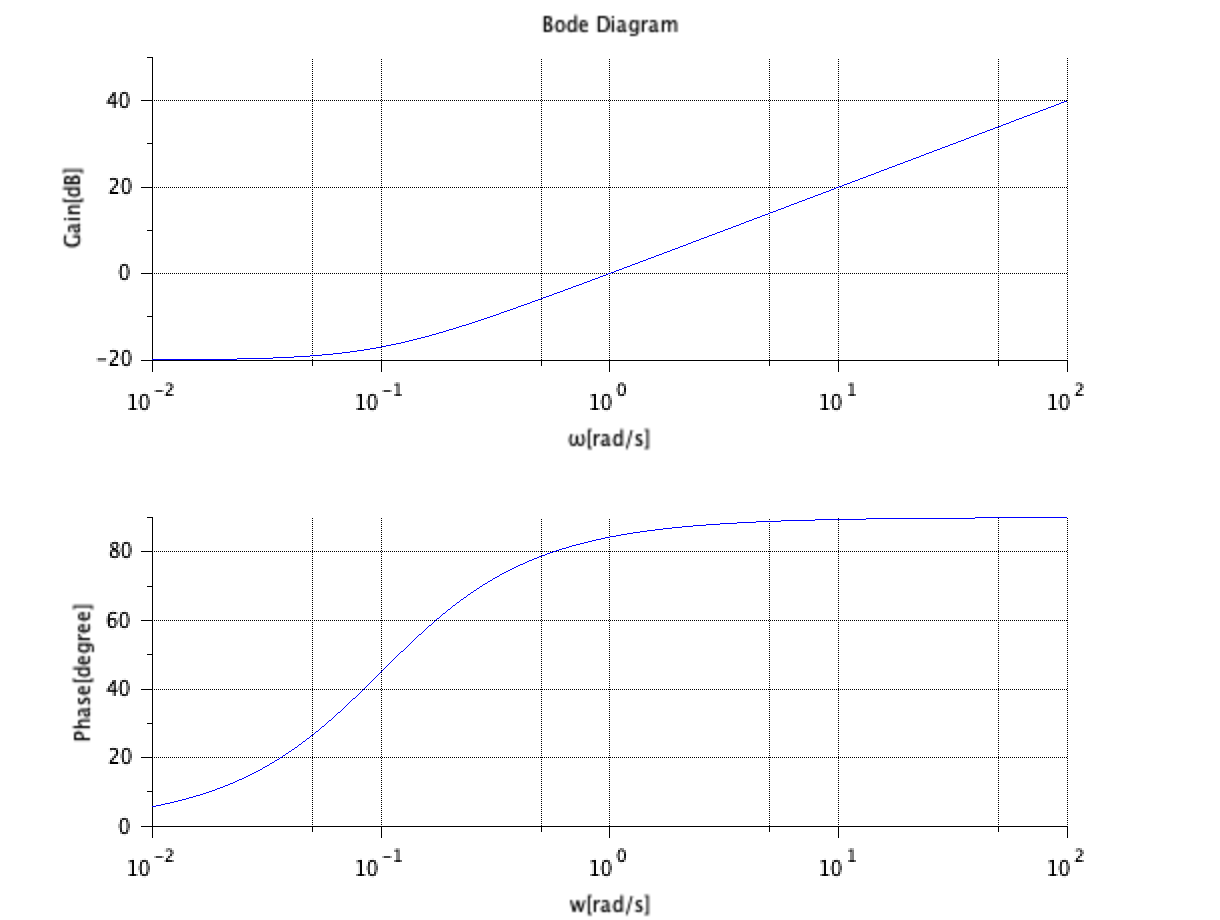
\includegraphics[width=0.8\linewidth]{picture/kadai7-3.png}
          \caption{$P_2(s)=s+0.1$のボード線図}
          \label{3-3-2-2-2}
        \end{figure}
  \item ボード線図上で$P_1(s)$と$P_2(s)$のゲイン曲線と位相曲線とを加え合わせると$P(s)$の
        それと一致することを確認する.\\
        以下に$P(s),P_1(s),P_2(s)$を一つの図にプロットする.以下にそのソースコードと
        実行結果(図\ref{3-3-2-3})示す.
        \begin{lstlisting}[caption=図\ref{3-3-2-3}をプロットするコード, label=C:3-3-2-3]
clear();
clc();
s=%s;

P=(s+0.1)/(s+1);
P1=1/s+1;
P2=s+0.1;

w = logspace(-2,2,400);

Pjw = horner(P,%i*w);
[Phase,GaindB] = phasemag(Pjw,'c');
P1jw = horner(P1,%i*w);
[Phase1,GaindB1] = phasemag(P1jw,'c');
P2jw = horner(P2,%i*w);
[Phase2,GaindB2] = phasemag(P2jw,'c');
scf(0);
xset('window',0);
subplot(211);
plot2d(w,GaindB, logflag='ln', style=2);
xtitle('Bode Diagram','ω[rad/s]','Gain[dB]')
xgrid();
subplot(212);
plot2d(w,Phase, logflag='ln', style=2);
xtitle('', 'w[rad/s]','Phase[degree]')
xgrid();

scf(1);
xset('window',1);
subplot(211);
plot2d(w,GaindB1, logflag='ln', style=2);
xtitle('Bode Diagram','ω[rad/s]','Gain[dB]')
xgrid();
subplot(212);
plot2d(w,Phase1, logflag='ln', style=2);
xtitle('', 'w[rad/s]','Phase[degree]')
xgrid();

scf(2);
xset('window',2);
subplot(211);
plot2d(w,GaindB2, logflag='ln', style=2);
xtitle('Bode Diagram','ω[rad/s]','Gain[dB]')
xgrid();
subplot(212);
plot2d(w,Phase2, logflag='ln', style=2);
xtitle('', 'w[rad/s]','Phase[degree]')
xgrid();

scf(3);
xset('window',3);
subplot(211);
plot2d(w,GaindB, logflag='ln', style=2);
xtitle('Bode Diagram','ω[rad/s]','Gain[dB]')
xgrid();
subplot(212);
plot2d(w,Phase, logflag='ln', style=2);
xtitle('', 'w[rad/s]','Phase[degree]')
xgrid();
xset('window',3);
subplot(211);
plot2d(w,GaindB1, logflag='ln', style=2);
xtitle('Bode Diagram','ω[rad/s]','Gain[dB]')
xgrid();
subplot(212);
plot2d(w,Phase1, logflag='ln', style=2);
xtitle('', 'w[rad/s]','Phase[degree]')
xgrid();
xset('window',3);
subplot(211);
plot2d(w,GaindB2, logflag='ln', style=2);
xtitle('Bode Diagram','ω[rad/s]','Gain[dB]')
xgrid();
subplot(212);
plot2d(w,Phase2, logflag='ln', style=2);
xtitle('', 'w[rad/s]','Phase[degree]')
xgrid();


xs2png(0, 'kadai7-1.png')
xs2png(1, 'kadai7-2.png')
xs2png(2, 'kadai7-3.png')
xs2png(3, 'kadai7-4.png')
      \end{lstlisting}
        \begin{figure}[H]
          \centering
          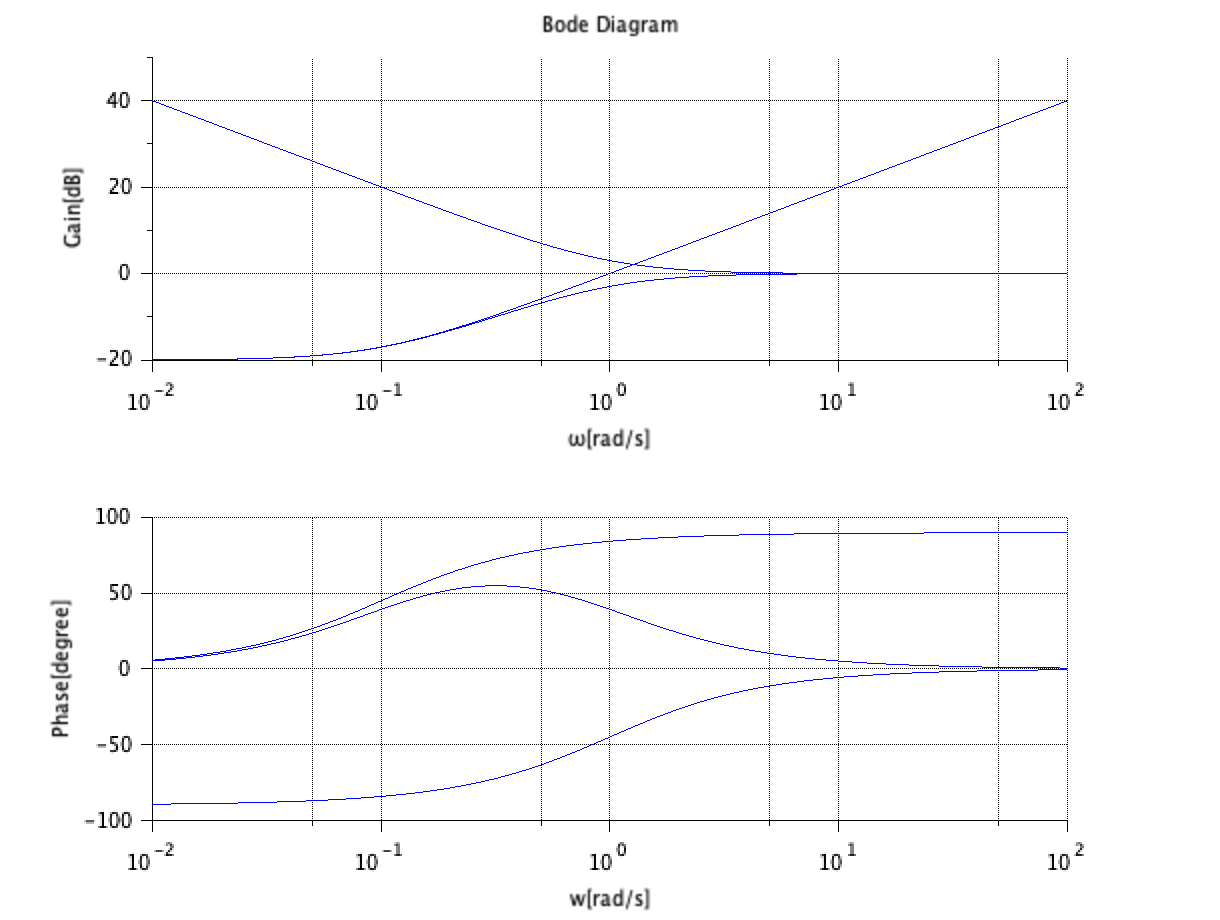
\includegraphics[width=0.8\linewidth]{picture/kadai7-4.png}
          \caption{$P(s),P_1(s),P_2(s)$のボード線図}
          \label{3-3-2-3}
        \end{figure}
\end{enumerate}

\section{研究課題}
\subsection{ゲイン位相線図について調べなさい}
ゲイン位相線図~\cite{gain}とは,ゲイン線図と位相線図を組み合わせたものである.
ゲイン線図とは,横軸に周波数の対数を取り,縦軸にゲイン(単位は$\si{\deci\bel}$)を取ったグラフを指す.
また,位相線図とは,横軸に周波数の対数を取り,縦軸に位相を取ったものである.
ゲイン位相線図を用いることにより,様々な周波数に対するシステムの特性を視覚的に表現することが
できることが最大の特徴である.

\subsection{一次遅れ系のナイキスト軌跡が円軌道を描くことを示しなさい}
一次遅れ系の式が以下の式\ref{ex1}と与えられたとする.
\begin{equation}
  G(s) = \frac{K}{Ts+1} \label{ex1}
\end{equation}
この式に,適当な$K,T$を代入して代入してどのようなグラフがプロットされるのかを確認する.以下のコード\ref{C:4-2}に
Scilabで作成したコードを示し,その実行結果を図\ref{G:4-2}に示す.なお,$K$は2,4,6と変化させ,
$T$は3,7,8と変化させた.
\begin{lstlisting}[caption=一次遅れ系のナイキスト軌跡, label=C:4-2]
clear;
clf;
scf(0);
s=%s;
P1 = syslin('c', 2/(3*s+1))
P2 = syslin('c', 4/(7*s+1))
P3 = syslin('c', 6/(8*s+1))
nyquist([P1;P2;P3],%t)
xs2png(0, 'ex4-2.png')
  \end{lstlisting}
\begin{figure}[H]
  \centering
  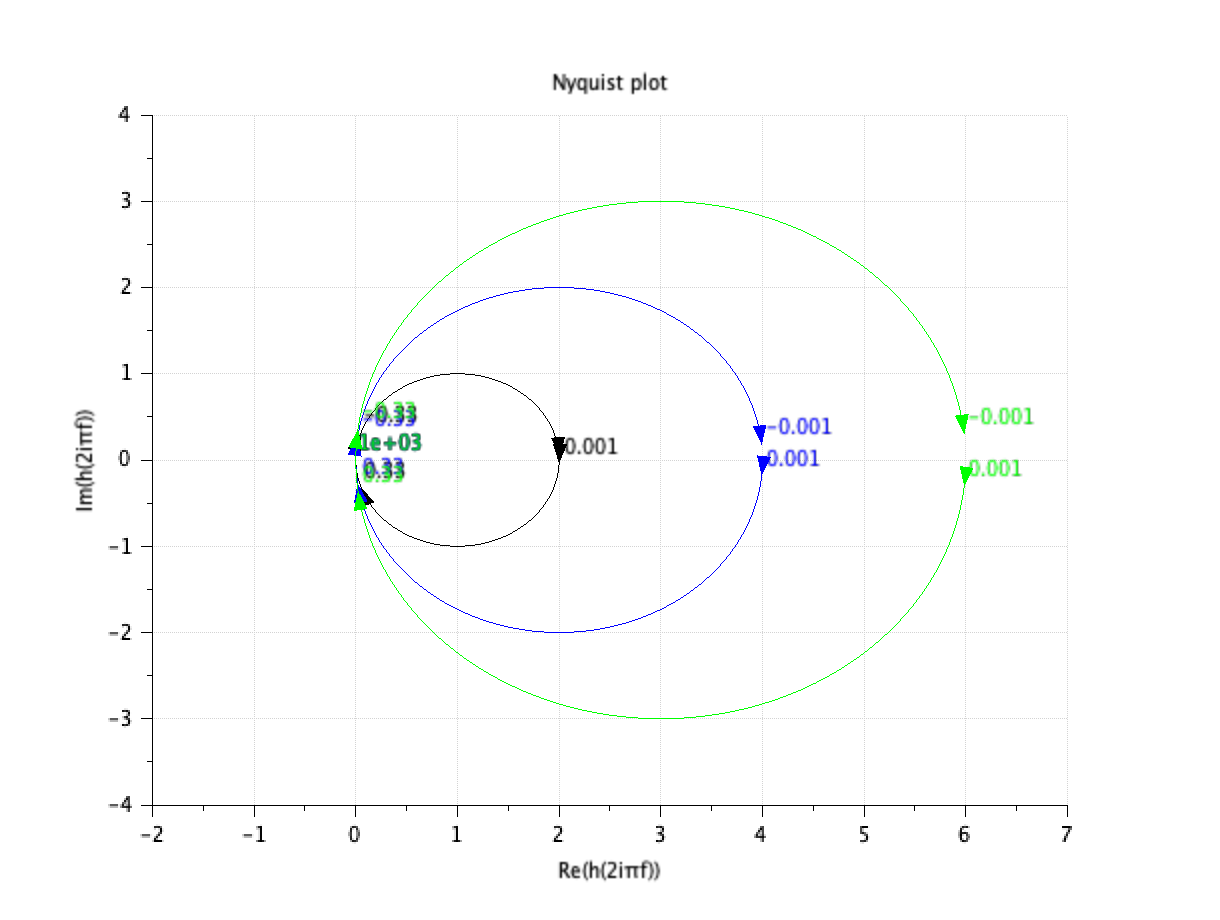
\includegraphics[width=0.8\linewidth]{picture/ex4-2.png}
  \caption{一次遅れ系のナイキスト軌跡}
  \label{G:4-2}
\end{figure}
以上より,一次遅れ系のナイキスト軌跡が円軌道を描くことがわかった.これについては考察にて式を導出する.

\section{考察}
研究課題で行った,一次遅れ系のナイキスト軌跡がなぜ円軌道を描くかについて考察する.\\
式\ref{ex1}の式において,$s=j\omega$のとき,\\
\begin{eqnarray}
  G(j\omega) &=& \frac{K}{j\omega T + 1} \nonumber \\
  &=& \frac{K(jT\omega)}{(jT\omega+1)(jT\omega-1)} \nonumber \\
  &=& \frac{K(1-jT\omega)}{T^2\omega^2+1} \nonumber \\
  &=& \frac{K}{T^2\omega^2}-j\frac{KT\omega}{T^2\omega^2+1}
\end{eqnarray}
と示すことができる.
ここで,$x = Re(G(j\omega))$,$y = In(G(j\omega))$と置くと,
\begin{eqnarray}
  x^2+y^2 &=& {\left(\frac{K}{T^2\omega^2}\right)}^2+{\left(\frac{KT\omega}{T^2\omega^2+1}\right)}^2 \nonumber \\
  &=& \frac{K^2+K^2T^2\omega^2}{(1+T^2\omega^2)^2} \nonumber \\
  &=& \frac{K^2(1+T^2\omega^2)}{(1+T^2\omega^2)^2} \nonumber \\
  &=& \frac{K^2}{1+T^2\omega^2} \nonumber \\
  &=& Kx \nonumber \\
  x^2 -Kx + y^2 &=& 0 \nonumber \\
  {\left(x - \frac{K}{2}\right)}^2  + y^2 &=& {\left(\frac{K}{2}\right)}^2 \label{Con1}
\end{eqnarray}
式\ref{Con1}より,中心から$+\frac{K}{2}$,半径$\frac{K}{2}$の円が描くことができることが導かれた.

\begin{thebibliography}{4}
  \bibitem{text} 永田 正伸 : 動的システムの周波数特性解析(周波数応答法):Scilab版 \\(制御情報システム工学 制御工学実験 指導書 2020年) \\
  \bibitem{junbi2} 数学活用大事典 :1次遅れ系の周波数応答の振幅 (最終閲覧日 2021年5月24日)\\ \url{http://omm.ishikawa-nct.ac.jp/ex/exercises/62idQAAC/#answer} \\
  \bibitem{gain} 理系大学院生の知識の森 : [ボード線図] ゲイン線図とは・書き方から学んで理解する,(最終閲覧日 2021年5月23日) \\\url{https://okasho-engineer.com/gain-diagram/}
\end{thebibliography}

\end{document}